% Template for PLoS
% Version 3.8 Apr 2026
% Adapted for: "A Multivariate Bayesian Framework for Diachronic Dating of
% Ancient Texts: Validation on Biblical Hebrew and Ancient Greek"

\documentclass[10pt,letterpaper]{article}
\usepackage[top=0.85in,left=2.75in,footskip=0.75in]{geometry}

\usepackage{amsmath,amssymb}
\usepackage{changepage}
\usepackage{textcomp,marvosym}
\usepackage{cite}
\usepackage{nameref,hyperref}
\usepackage[right]{lineno}
\usepackage[nopatch=eqnum]{microtype}
\DisableLigatures[f]{encoding = *, family = * }
\usepackage[table]{xcolor}
\usepackage{array}
\usepackage{booktabs}

\newcolumntype{+}{!{\vrule width 2pt}}

\newlength\savedwidth
\newcommand\thickcline[1]{%
  \noalign{\global\savedwidth\arrayrulewidth\global\arrayrulewidth 2pt}%
  \cline{#1}%
  \noalign{\vskip\arrayrulewidth}%
  \noalign{\global\arrayrulewidth\savedwidth}%
}
\newcommand\thickhline{\noalign{\global\savedwidth\arrayrulewidth\global\arrayrulewidth 2pt}%
\hline
\noalign{\global\arrayrulewidth\savedwidth}}

\raggedright
\setlength{\parindent}{0.5cm}
\textwidth 5.25in
\textheight 8.75in

\usepackage[aboveskip=1pt,labelfont=bf,labelsep=period,justification=raggedright,singlelinecheck=off]{caption}
\renewcommand{\figurename}{Fig}

\bibliographystyle{plos2025}

\makeatletter
\renewcommand{\@biblabel}[1]{\quad#1.}
\makeatother

\usepackage{lastpage,fancyhdr,graphicx}
\usepackage{epstopdf}
\pagestyle{fancy}
\fancyhf{}
\rfoot{\thepage/\pageref{LastPage}}
\renewcommand{\headrulewidth}{0pt}
\renewcommand{\footrule}{\hrule height 2pt \vspace{2mm}}
\fancyheadoffset[L]{2.25in}
\fancyfootoffset[L]{2.25in}
\lfoot{\today}

% Convenience macros
\newcommand{\bhsa}{\textsc{bhsa}}
\newcommand{\cbh}{CBH}
\newcommand{\lbh}{LBH}
\newcommand{\mvn}{MLE-MVN}
\newcommand{\hbvi}{HB-VI}
\newcommand{\Smat}{\boldsymbol{\Sigma}}
\newcommand{\muvec}{\boldsymbol{\mu}}
\newcommand{\xvec}{\mathbf{x}}
\newcommand{\bvec}{\boldsymbol{\beta}}


\begin{document}
\vspace*{0.2in}

\begin{flushleft}
{\Large
\textbf{A multivariate Bayesian framework for diachronic dating of ancient
texts: Validation on Biblical Hebrew and Ancient Greek}
}
\newline
\\
Aaron Adair\textsuperscript{1*}
\\
\bigskip
\textbf{1} Department of Physics, Massachusetts Institute of Technology, Cambridge, MA, USA
\\
\bigskip
* Corresponding author: adairaar@mit.edu

\end{flushleft}

% -------------------------------------------------------
\section*{Abstract}
% -------------------------------------------------------

Linguistic dating of ancient texts --- inferring composition date from
internal morphosyntactic evidence --- is central to biblical studies,
classical philology, and Near Eastern linguistics, yet it has rarely been
formalized as a probabilistic inference problem.  Existing approaches
identify features that shift between early and late corpora and assign
ordinal labels (``archaic,'' ``late''), but they do not produce calibrated
probability distributions over dates.  We present a framework that addresses
this gap.

The core model (\mvn{}) fits an ordinary-least-squares regression per
morphosyntactic feature against date, assembles the residual covariance
with Tikhonov (ridge) regularization, and evaluates a multivariate normal
log-likelihood over a fine date grid to obtain a proper Bayesian posterior.
A companion hierarchical Bayesian model with variational inference
(\hbvi{}) extends this with group-level shrinkage and Monte Carlo
uncertainty propagation, yielding better-calibrated credible intervals and
enabling soft register assignment.

Three confound-correction modules are introduced: (1) a \emph{resistant
model} using only four clause-level syntactic features below conscious
editorial control, providing an archaism diagnostic; (2) a \emph{genre
correction} (Strategies B+D) that down-weights features driven by legal
versus narrative register rather than by date; and (3) a \emph{word n-gram
model} using POS-tag and function-word sequence features as an independent
grammatical-sequence dating check.

The framework is trained on 22 prophetic and post-exilic Hebrew texts with
independent historical anchoring (760--167~BCE) drawn from the Biblia
Hebraica Stuttgartensia Amstelodamensis (\bhsa{}) database.  Held-out
validation on oracle Jeremiah chapters (never seen in training) returns
MAP~=~562~BCE with mean LBH score~=~0.16, consistent with a 7th-century
text.  \hbvi{} achieves holdout MAE of 16.8~yr versus 134.2~yr for
\mvn{} on three chronologically anchored holdouts.  Cross-language
validation on a 63-text Ancient Greek corpus (five holdouts) recovers all
MAP dates within $\sim$30~yr of established scholarly dates, demonstrating
that the methodology is language-agnostic.  All code and corpora are
publicly available (see Data Availability).

% -------------------------------------------------------
\clearpage
\newgeometry{top=0.85in,left=1in,right=1in,footskip=0.75in}
\linenumbers

% -------------------------------------------------------
\section*{Introduction}
% -------------------------------------------------------

Scholars in biblical studies, classical philology, and Near Eastern
linguistics routinely use internal linguistic evidence to constrain the
dates of ancient texts.  The transition from Classical Biblical Hebrew
(\cbh{}) to Late Biblical Hebrew (\lbh{}) is among the best-documented
diachronic shifts in any ancient language~\cite{Hurvitz1982,Rooker1990,
Polzin1976}, and comparable transitions are well attested in Ancient
Greek~\cite{Horrocks2010} and Akkadian.  Despite this rich empirical
tradition, linguistic dating almost never produces calibrated probability
estimates; scholars identify features as ``archaic'' or ``late'' and
assign texts to qualitative categories, but the resulting claims carry no
quantified uncertainty.

A notable recent contribution by Faigenbaum-Golovin et al.~\cite{Faigenbaum2025}
demonstrated that statistical analysis of lemma n-gram frequencies can
reliably distinguish among the three major scribal corpora of the Hebrew
Bible --- the old layers of Deuteronomy (D), the Deuteronomistic History
(DtrH), and the Priestly source (P) --- achieving approximately 84\%
chapter-level attribution accuracy on a 50-chapter benchmark, with
interpretable discriminating-lemma lists linking computational results to
traditional philological categories.  That study establishes the viability
of quantitative computational methods for biblical Hebrew scholarship and
demonstrates that linguistically distinct scribal schools leave detectable
statistical fingerprints even in relatively short texts.  Its focus,
however, is \emph{authorship attribution}: given a passage of disputed
origin, which known scribal milieu produced it?  The present paper
addresses the complementary but methodologically distinct question of
\emph{diachronic dating}: not ``which school wrote it?'' but ``when was it
written?''  These are related but separable questions that demand different
statistical frameworks, different feature sets, and different validation
strategies, as detailed below.

This paper addresses two methodological gaps that authorship-attribution
approaches leave open.  First, no existing probabilistic framework
provides date posteriors with credible intervals for Biblical Hebrew texts.
Qualitative assessments of individual features are genuinely informative,
but they cannot be combined into a single coherent posterior without a
model that propagates feature-level evidence into a joint probability
distribution over dates.  Second, no principled framework separates the
temporal signal from two well-known confounds:
\emph{archaism} (a late composer deliberately employing archaic vocabulary
and morphology) and \emph{genre} (legal or narrative register producing
feature distributions that mimic either earlier or later stages of the
language independently of composition date).

The framework presented here makes the following contributions:
\begin{enumerate}
  \item A morphosyntactic feature extraction pipeline operating on the
    \bhsa{}/\textsc{etcbc} database~\cite{BHSA2021,Roorda2018}, producing
    35 features across three tiers (lexical, morphological, and
    clause-level syntactic), selected by Spearman correlation ($p < 0.30$)
    with 100\% LOO sign-consistency.
  \item The \mvn{} Bayesian dating model: per-feature OLS regression,
    Tikhonov-regularized residual covariance, and posterior over a
    500-point date grid with explicit uncertainty quantification.
  \item The \hbvi{} model: hierarchical Bayesian regression with
    mean-field variational inference (MFVI) and ADAM
    optimization~\cite{Kingma2014,Blei2017}, providing proper parameter
    uncertainty propagation and soft register assignment.
  \item A resistant model using only four clause-level features below
    conscious editorial control, yielding an archaism diagnostic from the
    divergence between the full and resistant MAP dates.
  \item Genre correction (Strategies B+D) that down-weights features
    according to their sensitivity to legal versus narrative register.
  \item A word n-gram model (POS-tag and function-word bigrams/trigrams)
    as an independent grammatical-sequence dating instrument.
  \item Prior sensitivity analysis distinguishing data-driven from
    prior-dominated \hbvi{} date estimates.
  \item Cross-language validation on a 63-text Ancient Greek corpus.
\end{enumerate}

The paper is organized as follows.  The Background section reviews the
CBH/LBH distinction and the methodological debates surrounding linguistic
dating.  The Data section describes the training corpus and feature
extraction.  The MLE-MVN and HB-VI sections present the two Bayesian
models.  The Prior Sensitivity Analysis section covers the three-mode
sensitivity framework.  The Archaism Detection section presents the
resistant model and archaism diagnostic.  The Genre Correction section
describes Strategies B+D.  The Validation section reports holdout and
cross-language results.  The Discussion section addresses limitations,
extensibility, and the relationship to authorship-attribution
approaches.

% -------------------------------------------------------
\section*{Background: diachronic Biblical Hebrew}
% -------------------------------------------------------

\subsection*{The CBH/LBH distinction}

Classical Biblical Hebrew (\cbh{}) is the language of the pre-exilic
prophetic corpus and early narrative material (8th--7th centuries BCE):
Amos, Hosea, early Isaiah, and the narrative strands of Samuel-Kings.
Late Biblical Hebrew (\lbh{}) characterizes the post-exilic prose of
Ezra, Nehemiah, Chronicles, Esther, and Daniel (5th--2nd centuries BCE).

The transition is marked by well-studied lexical, morphological, and
syntactic changes~\cite{Hurvitz1997,Rooker1990,Polzin1976}.  At the
lexical level, the first-person singular pronoun shifts from \textit{ank\={\i}}
(\textsc{cbh}) to \textit{an\={\i}} (\textsc{lbh}); the relative
pronoun \textit{ašer} gives way to the enclitic \textit{š}e-; the negator
\textit{l\={o}\textquotesingle} is supplemented by and eventually partly
replaced by \textit{\textquotesingle \={e}n}.  At the morphological level,
the wayyiqtol (narrative imperfect) declines in frequency while the
\textit{h\={a}y\={a}h} + participle periphrastic progressive increases.
At the syntactic level, infinitive-absolute constructions rise, and the
overall sentence structure shifts toward the analytic patterns associated
with Aramaic influence~\cite{Young2008,Rezetko2014}.

The consensus view~\cite{Hurvitz1982,Hurvitz2014,Robertson1972} holds that
these features shift monotonically along the temporal axis, constituting a
reliable if noisy diachronic signal.  The present study adopts this view as
a working assumption while formally modeling and partially testing the
alternatives.

\subsection*{The diachronic versus dialectal debate}

Young, Rezetko, and Ehrensv\"{a}rd~\cite{Young2008} argue that the CBH/LBH
contrast may reflect geographic dialect, scribal tradition, or literary
register rather than chronology.  The Qumran sectarian texts (Dead Sea
Scrolls, $\sim$150~BCE) deliberately employ \cbh{} vocabulary and
morphology while simultaneously using Aramaic loan-words --- a pattern
interpreted as literary register rather than temporal reality.

Hurvitz and the diachronic mainstream~\cite{Hurvitz1997} counter that the
dialectal alternatives require additional auxiliary hypotheses; and that
the Qumran archaism case presupposes the original \cbh{} features had
already receded, confirming rather than undermining the diachronic
interpretation.

Crucially for the present paper: rather than adjudicating this debate
purely on a priori grounds, the framework operationalizes it.  The
\emph{resistant model} tests whether syntactic templating patterns that
fall below the level of deliberate stylistic choice agree with the
full-model (lexical + morphological + syntactic) date.  Systematic
disagreement --- the full model older than the resistant model --- is a
falsifiable indicator of archaism.

\subsection*{The circularity problem}

Dating methods that use features identified by comparing texts of assumed
date risk circularity: the assumed dates shape the feature set, and the
feature set is then used to infer unknown dates.  We adopt three
safeguards.

First, the training corpus is restricted to prophetic books with
\emph{independent} historical anchoring via synchronisms with datable
rulers in Assyrian, Babylonian, and Persian king-lists.  Torah texts
are excluded from training entirely, so all Torah date estimates are
genuine out-of-sample predictions.

Second, a held-out validation set (oracle Jeremiah chapters) was
withheld from all feature selection and training.  Its correct recovery by
the model (Section~9) provides empirical evidence against the circularity
objection.

Third, the prior sensitivity analysis (Section~6) explicitly quantifies
how much of each \hbvi{} date is determined by the scholar-specified
prior versus the linguistic data.

Beyond these three safeguards, the choice of the prophetic corpus as the
training base deserves explicit justification, and the \emph{direction} of
any residual misdating error is methodologically important.

\textbf{Why the prophetic corpus.}
The Hebrew prophetic books offer a form of historical anchoring available
nowhere else in the Hebrew Bible: their superscriptions and internal
chronological notices can be cross-checked against records entirely external
to the biblical tradition.  Ezekiel explicitly dates thirteen of his visions
to regnal years of the Babylonian exile --- ``the fifth year of King
Jehoiachin's captivity'' (Ezek~1:2), ``the sixth year'' (8:1), and so
forth --- which can be correlated with Babylonian administrative texts that
independently date Jehoiachin's deportation to~597~BCE.  Other eighth-
and seventh-century prophets (Amos, Hosea, Isaiah, Micah, Zephaniah,
Nahum) are anchored by superscriptions naming Judahite and Israelite kings
whose reigns are independently documented in the Assyrian and
Neo-Babylonian annals.  No comparable external anchoring exists for the
Torah or the poetic books: their dates are derived entirely from
literary-critical arguments, which is precisely the kind of circularity the
present study seeks to avoid.  The prophetic corpus therefore represents
the most defensible choice for a training set whose dates are genuinely
independent of the linguistic features under analysis.

\textbf{Asymmetric error and conservative upper limits.}
If the accepted dates for the prophetic training texts were wrong, the
error would be asymmetric: these texts can be \emph{no older} than the
historical events they reference (the superscriptions and Ezekielian dates
provide firm termini post quos), but they could in principle be
\emph{younger} --- composed or reaching final form some time after the
events they describe.  This asymmetry has a direct consequence for the
date estimates produced by the model.  A training corpus that is misdated
in the direction of being too early would calibrate the feature-to-date
mapping at too early a point on the temporal axis; unknown texts dated
by reference to that calibration would also be estimated as too early,
meaning their true dates would be \emph{later} than the model reports.
In other words, if the prophetic training dates carry any systematic error,
that error propagates in a single direction: all model-derived dates shift
toward greater recency, not greater antiquity.  The model's output for a
text such as the Song of the Sea --- already placed firmly in the Persian
period by the resistant model --- would be pushed later still if the
training corpus were found to be younger than traditionally assumed.  The
dates reported in this study should therefore be understood as
\emph{conservative upper bounds on antiquity}: a text dated here to
400~BCE may be more recent, but the linguistic evidence as calibrated
against the prophetic corpus provides no support for a date earlier than
that estimate.

% -------------------------------------------------------
\subsection*{Prior computational work: authorship attribution versus
diachronic dating}
% -------------------------------------------------------

Faigenbaum-Golovin et al.~\cite{Faigenbaum2025} provide the most
methodologically rigorous prior computational treatment of the Hebrew Bible.
Their Higher Criticism (HC) discrepancy method~\cite{Faigenbaum2025} tests
whether the distribution of lemma n-gram frequencies in a target text
deviates from the null hypothesis that it was produced by the same process
as a reference corpus.  Applied to 50 ground-truth chapters spanning D,
DtrH, and P, the method achieves 84\% attribution accuracy in leave-one-out
validation and yields interpretable discriminating-lemma lists that directly
engage traditional philological categories.  The statistical
optimality properties of the HC statistic (sensitivity to rare but
consistent frequency deviations across a large vocabulary) make it
well-suited to its task.

The present framework is designed to answer a different question, and five
methodological consequences follow directly from that distinction.

\textbf{Continuous date posteriors versus categorical corpus assignment.}
The HC method assigns each text to the most likely of three corpora.
Because D and DtrH are both dated to the late monarchic or exilic period,
two texts composed at 650 and 590~BCE receive identical labels if both
score closest to DtrH; no intra-school temporal resolution is possible.
The \mvn{} and \hbvi{} models instead compute a posterior probability
distribution over a 500-point continuous date grid, recovering whatever
temporal resolution the data support and quantifying uncertainty explicitly
via credible intervals.

\textbf{Morphosyntactic features versus raw lemma frequencies.}
Faigenbaum-Golovin et al.\ operate on raw lemma and lemma n-gram
frequencies --- a bag-of-words representation in which content words
(e.g., \textit{gold} in Tabernacle chapters, \textit{king} in regnal
narratives) dominate the signal.  Content-word frequencies are sensitive
to \emph{topic} and \emph{genre} as much as to \emph{authorship}, and
they carry little temporal signal for cross-genre comparisons.  The 36
features used in this study are drawn from a century of diachronic Hebrew
linguistics scholarship~\cite{Hurvitz1982,Polzin1976,Rooker1990,Young2008}
precisely because they are sensitive to \emph{period} rather than
\emph{topic}: the \textit{ank\={\i}}$\to$\textit{an\={\i}} pronoun shift,
the negator transition, the wayyiqtol decline, and the
infinitive-absolute rate change systematically across time and resist
topical or generic influence.  This distinction is especially important
for cross-genre comparisons: bag-of-words features cannot compare poetic
or legal texts against narrative texts without large genre confounds.

\textbf{Archaism diagnostic.}
The HC method provides no mechanism for distinguishing a genuinely ancient
text from one composed in a deliberately archaic register.  A Persian-period
author who archaizes vocabulary to D/DtrH norms will be assigned to
DtrH regardless of actual composition date.  The resistant/full-model
divergence introduced in Section~7 detects this pattern directly: surface
features under conscious compositional control (lexicon, morphology) and
deep clause-level syntactic patterns that operate below deliberate stylistic
choice are evaluated independently, and systematic divergence between their
date estimates constitutes a quantified, falsifiable indicator of archaism.
This diagnostic has no counterpart in the HC framework.

\textbf{External holdout validation.}
Faigenbaum-Golovin et al.\ validate via leave-one-out and $k$-fold
cross-validation within the three training corpora.  This confirms internal
consistency but cannot test whether the method recovers \emph{correct}
calendar dates, because the ground-truth labels are scribal-school
assignments rather than independently anchored absolute dates.  The present
framework is validated against texts anchored to external historical events
--- oracle Jeremiah chapters to the Neo-Babylonian
period~\cite{Hurvitz1999}, Haggai to 520~BCE (Persian regnal date),
Daniel Hebrew chapters to 167~BCE (Maccabean crisis) --- providing a
genuinely independent test that the temporal signal is real rather than
self-referential.

\textbf{Cross-linguistic generalization.}
The Greek validation corpus (63 texts, five held-out texts spanning Archaic
through Byzantine Greek) demonstrates that the methodology captures a
general diachronic morphosyntactic signal and does not exploit properties
idiosyncratic to Biblical Hebrew.  No cross-linguistic generalization of
the HC authorship method has been reported.

These five differences are differences of purpose rather than
deficiencies in either approach.  Authorship attribution and diachronic
dating ask related but separable questions; the ideal analysis of any
disputed text would apply both.  The HC output (scribal-school membership)
can in principle be used to set register priors in \hbvi{}, and
conversely \hbvi{} date posteriors constrain the plausible compositional
settings for HC attribution decisions.  We return to this complementarity
in the Discussion.

% -------------------------------------------------------
\section*{Data: corpus and feature extraction}
% -------------------------------------------------------

\subsection*{The BHSA database}

All Hebrew text analysis uses the Biblia Hebraica Stuttgartensia
Amstelodamensis (\bhsa{}) database, version 2021, produced by the Eep
Talstra Centre for Bible and Computer (ETCBC) at Vrije Universiteit
Amsterdam~\cite{BHSA2021,Roorda2018,Roorda2014}.  \bhsa{} provides
morphological tagging at the word level, phrase-level function annotation,
clause boundary segmentation, and lexeme coding for the entire Hebrew
Bible.  Data are accessed programmatically via the Text-Fabric Python
library, enabling reproducible extraction without manual annotation.  No
Aramaic chapters are included in training or testing.

\subsection*{Training corpus}

The training corpus comprises 22 prophetic and post-exilic prose units
spanning 760--167~BCE (Table~\ref{tab:corpus}).  Date anchoring uses
explicit synchronisms with datable ancient Near Eastern events: for
example, Amos~1:1 places the book in the reigns of Uzziah and Jeroboam~II
($\sim$760~BCE); Haggai~1:1 gives an explicit Persian regnal date
(520~BCE); Daniel's Hebrew chapters~(1,~8--12) are anchored to
167~BCE by the Maccabean crisis.

Several calibration decisions require note.  Isaiah~56--66 (Trito-Isaiah)
is set at 450~BCE, reflecting scholarly near-consensus for Persian-period
composition.  Ezra and Nehemiah are set at 350~BCE, reflecting arguments
for late-Persian or early Hellenistic final form.  Daniel is restricted
to Hebrew chapters~1 and~8--12; the Aramaic chapters~(2--7) are a different
language and are excluded.

Oracle Jeremiah chapters (the oracular stratum: chs.~1--6, 8--10, 12--16,
19--20, 22--23, 30--31, 46--51) and the Deuteronomistic prose stratum
(chs.~7, 11, 17--18, 21, 24--29, 32--45, 52) are both excluded from
training and used exclusively as held-out validation units.

\begin{table}[!ht]
\centering
\caption{\textbf{Training corpus: 22 units with anchored dates and word
counts.}  Date (BCE) is the scholarly consensus midpoint used as the
training label.  $\sigma$ is the uncertainty estimate fed to the HB-VI
prior.  Register: S = SBH, T = Transitional, L = LBH.}
\begin{tabular}{llrrr}
\hline
\textbf{Unit} & \textbf{Register} & \textbf{Date (BCE)} &
  \textbf{$\sigma$ (yr)} & \textbf{Words} \\
\hline
Amos           & S & 760 & 20 & 2{,}042 \\
Hosea          & S & 745 & 20 & 2{,}971 \\
Micah          & S & 725 & 20 & 1{,}786 \\
Isaiah 1--39   & S & 720 & 30 & 8{,}241 \\
Nahum          & S & 650 & 20 & 618  \\
Habakkuk (training) & S & 605 & 20 & 670 \\
Zephaniah      & S & 630 & 20 & 1{,}009 \\
Jeremiah oracle& S & 605 & 30 & 11{,}842 \\
Ezekiel        & T & 580 & 20 & 18{,}793 \\
Isaiah 40--55  & T & 545 & 20 & 4{,}951 \\
Isaiah 56--66  & T & 450 & 30 & 2{,}808 \\
Obadiah        & T & 580 & 30 & 291  \\
Joel           & T & 400 & 50 & 1{,}060 \\
Jonah          & T & 400 & 50 & 687  \\
Malachi        & T & 460 & 20 & 913  \\
Zechariah 1--8 & T & 518 & 10 & 2{,}302 \\
Zechariah 9--14& L & 350 & 50 & 1{,}538 \\
Ezra           & L & 350 & 30 & 4{,}092 \\
Nehemiah       & L & 350 & 30 & 5{,}784 \\
Esther         & L & 300 & 50 & 3{,}122 \\
Chronicles     & L & 330 & 30 & 25{,}946 \\
Daniel (Heb.)  & L & 167 & 10 & 3{,}041 \\
\hline
\end{tabular}
\label{tab:corpus}
\end{table}

\subsection*{Feature extraction}

Features are extracted at three tiers that differ in their susceptibility
to deliberate stylistic manipulation (Table~\ref{tab:features}).

\textbf{Tier~1 (lexical, 20 features).}  Rates per 1{,}000 words of
specific function words, particles, demonstratives, and prepositions.
Examples: the \textit{ašer}/\textit{š}e ratio; the \textit{ank\={\i}}/\textit{an\={\i}}
ratio; the absolute rate of the particle \textit{gam}; the rate of the
accusative marker \textit{et}.  Tier~1 features most directly capture the
\cbh{}/\lbh{} lexical axis but are also most susceptible to deliberate
archaism, because a competent composer can deliberately choose archaic
function words.

\textbf{Tier~2 (morphological, 12 features).}  Verb stem fractions
(qal, piel, hif, niphal as fractions of all verbs); verb form fractions
(wayyiqtol, qatal, yiqtol, participle, imperative fractions); absolute noun
ratio; pronominal suffix rate.  These are harder to archaize wholesale but
remain subject to word-level editorial manipulation.

\textbf{Tier~3 (clause/phrase, 4 features).}  Four features forming the
\emph{resistant model}: the infinitive-construct fraction (\texttt{frac\_infc}),
the fronted-clause fraction (\texttt{frac\_fronted}), the null-subject
fraction (\texttt{frac\_null\_subj}), and the waw-qatal fraction
(\texttt{frac\_wqtl\_wayq}).  These measure syntactic templating patterns
that are acquired below the level of conscious stylistic choice and are
therefore most resistant to deliberate manipulation.

\textbf{Feature selection.}  Spearman rank correlation with date is
computed for each candidate feature against the 22-text training set.
Features are retained at a permissive significance threshold of $p < 0.30$:
with only $N = 22$ training texts, a strict Benjamini-Hochberg FDR
correction at $\alpha = 0.05$ would retain only $\sim$10 features, which
is insufficient to capture the multi-dimensional CBH/LBH signal documented
over a century of Hebrew linguistics scholarship.  The $p < 0.30$ threshold
is paired with a leave-one-out (LOO) robustness filter: a feature is
retained only if its Spearman $\rho$ preserves sign in $\geq 68\%$ of LOO
resamplings (the 68\% threshold corresponds to one standard deviation of a
binomial sign-consistency test, providing a principled stopping criterion).
In practice, all 35 features surviving the $p < 0.30$ screen achieve
100\% LOO sign consistency (LOO fraction $= 1.00$), well above the 68\%
floor, confirming that the selected features carry a robust diachronic
signal.  This yields a final set of \textbf{35 features}.

\begin{table}[!ht]
\centering
\caption{\textbf{Feature tier summary.}  J = number of features in tier.
Susceptibility indicates the degree to which deliberate archaism can
manipulate features within that tier.}
\begin{tabular}{llll}
\hline
\textbf{Tier} & \textbf{Type} & \textbf{J} & \textbf{Archaism susceptibility} \\
\hline
1 & Lexical (function words, particles) & 20 & High \\
2 & Morphological (verb forms, stems)   & 12 & Medium \\
3 & Clause/phrase syntax                &  4 & Low (resistant model) \\
\hline
\multicolumn{2}{l}{Total selected} & 35 & \\
\hline
\end{tabular}
\label{tab:features}
\end{table}

\subsection*{Word n-gram model}

As an independent grammatical-sequence dating instrument, we extract
POS-tag n-gram features that are immune to topic variation and largely
immune to deliberate lexical archaism: a composer can choose archaic
vocabulary but cannot easily rewrite every grammatical-sequence pattern
to match an earlier era.

Two feature types are used.  \textbf{Type~A} features are POS-tag bigrams
and trigrams on all words (e.g., \texttt{verb\_wayyiqtol\,\textperiodcentered\,noun},
\texttt{prep\,\textperiodcentered\,prps}), capturing deep grammatical flow.
\textbf{Type~B} features are function-word lexeme bigrams and trigrams
restricted to seven closed-class POS categories (prepositions, conjunctions,
articles, negators, personal pronouns, demonstratives, interrogatives),
making them robust to both topic and rare-vocabulary variation.  The combined
A+B model (\texttt{MAP\_AB}) uses 56 features and is the primary word n-gram
estimate reported in all tables.

\textbf{Character n-gram model: assessment and exclusion.}  An earlier
version of the framework included character 3-gram and 4-gram frequencies.
Reliability testing on 1QS (Community Rule, Dead Sea Scrolls;
independently dated $\sim$150~BCE) returned MAP~=~760~BCE --- a 600-year
error attributable to deliberate orthographic archaism.  Sub-morphemic
patterns are not immune to deliberate archaism in the Biblical Hebrew
corpus.  The character n-gram model is therefore excluded from all
analyses; this negative result is reported because it is informative about
the limits of the approach.

% -------------------------------------------------------
\section*{The MLE-MVN model}
% -------------------------------------------------------

\subsection*{Per-feature OLS regression}

Each feature $f_j$ ($j = 1, \ldots, J$, $J = 35$) is modeled as a linear
function of date $d$ plus Gaussian noise:
%
\begin{equation}
  f_j(d) = \alpha_j + \beta_j \, d + \varepsilon_j, \qquad
  \varepsilon_j \sim \mathcal{N}(0, \sigma_j^2).
  \label{eq:ols}
\end{equation}
%
Parameters $(\hat{\alpha}_j, \hat{\beta}_j)$ are estimated by OLS on the
22-unit training corpus.  The predicted feature vector at date $d$ is
$\muvec(d) = \hat{\alpha}_j + \hat{\beta}_j d$ stacked over $j$.

The linear model is a simplification: some features (e.g., wayyiqtol
fraction) may have mild non-linear trends.  A sensitivity analysis with
quadratic terms shows negligible improvement over the date range
760--167~BCE, justifying the linear approximation.

\subsection*{Tikhonov-regularized residual covariance}

The $J \times J$ residual covariance matrix $\Smat$ captures co-variation
among features unexplained by the date trend.  Because the training
corpus has only $N = 22$ units, $\Smat$ estimated from the raw residuals
is near-singular when $J = 35$.  Tikhonov (ridge) regularization is
applied:
%
\begin{equation}
  \Smat_{\text{reg}} = \Smat +
    \lambda \cdot \frac{\mathrm{tr}(\Smat)}{J} \, \mathbf{I}_J,
  \label{eq:ridge}
\end{equation}
%
where $\lambda = 0.10$ for the full model and $\lambda = 0.20$ for the
resistant model (four features only).  A sensitivity analysis varying
$\lambda \in [0.05, 0.30]$ shows MAP estimates stable to $\pm 30$~yr
across representative training and holdout texts.  As expected, 68\%
credible interval widths increase monotonically with $\lambda$, growing
by 50--70~yr over the tested range (from $\sim$110--135~yr at
$\lambda = 0.05$ to $\sim$160--200~yr at $\lambda = 0.30$), reflecting
the trade-off between regularization stability and posterior confidence.
The canonical value $\lambda = 0.10$ was chosen to balance near-singular
covariance suppression against excessive CI widening.

\subsection*{Posterior computation}

A 500-point date grid spanning 900~BCE to 100~CE (step $\approx 2$~yr)
is evaluated.  The log-likelihood of observed feature vector $\xvec$
at grid point $d$ is
%
\begin{equation}
  \ell(d) = -\tfrac{1}{2}
    \bigl(\xvec - \muvec(d)\bigr)^{\!\top}
    \Smat_{\text{reg}}^{-1}
    \bigl(\xvec - \muvec(d)\bigr).
  \label{eq:loglik}
\end{equation}
%
A weakly informative Gaussian prior $p(d) = \mathcal{N}(464, 300^2)$
(centered at the training midpoint) is added in log space, and the result
is normalized to a proper posterior:
%
\begin{equation}
  p(d \mid \xvec) \;\propto\; \exp\bigl\{\ell(d)\bigr\} \cdot p(d).
  \label{eq:posterior}
\end{equation}
%
The MAP estimate is the mode; 68\% and 95\% highest-density credible
intervals (HDCIs) are extracted numerically.

% -------------------------------------------------------
\section*{The HB-VI model}
% -------------------------------------------------------

\subsection*{Motivation and limitations of MLE-MVN}

The \mvn{} model treats each feature regression independently and uses
point estimates for all parameters.  Two failure modes motivate the
hierarchical extension.  First, the resulting 68\% CIs are extremely
narrow (median 3--4~yr for SBH texts), indicating the model is
systematically overconfident; parameter uncertainty in $\hat{\beta}_j$
is not propagated.  Second, register assignment is hard: a text must be
pre-assigned to one of three groups (SBH/Transitional/LBH) before the
posterior is computed.  Misassignment cascades into catastrophically
wrong dates (e.g., Haggai assigned to LBH: MAP~=~361~BCE vs.\ 520~BCE
actual; error~=~159~yr; holdout MAE for \mvn{}~=~134~yr).

\subsection*{Hierarchical model architecture}

The \hbvi{} model is a hierarchical Bayesian regression in which
per-group feature loadings are drawn from a global distribution:
%
\begin{equation}
  \beta_{r,j} \sim \mathcal{N}(\mu_{\beta_j},\, \sigma_\beta^2),
  \label{eq:hbvi_prior}
\end{equation}
%
where $r \in \{1,2,3\}$ indexes the register group (SBH, Transitional,
LBH), $j$ indexes the feature, and $\mu_{\beta_j}$ and $\sigma_\beta$ are
global hyperparameters shared across groups.  Groups share statistical
strength via the global hyperparameters while maintaining group-specific
slopes.  Intercepts $\alpha_{r,j}$, noise variance $\sigma_{r,j}$, and
the global hyperparameters are all variational parameters.

The training corpus for the \hbvi{} model uses 19 texts (7 SBH,
6 Transitional, 6 LBH), with the three holdout texts (Habakkuk, Haggai,
Daniel) excluded, and the full Jeremiah book replaced by the oracle Jeremiah
chapters as the SBH anchor.  Date priors for training texts are
$\mathcal{N}(d_{\text{BCE}}, \sigma_{\text{date}}^2)$, directly encoding
known date uncertainty.

\subsection*{Variational inference training}

Rather than sampling the full posterior directly (which is computationally
prohibitive for a hierarchical model of this size), we fit a simpler
parametric approximation to it.  Specifically, we choose an independent
Gaussian distribution for each model parameter and optimize its mean and
variance to match the true posterior as closely as possible.  This
approach---mean-field variational inference (MFVI)---converts Bayesian
inference into an optimization problem, making it tractable on a standard
laptop without GPU hardware.

Formally, the posterior $p(\boldsymbol{\theta} \mid \mathbf{X})$ is approximated
by mean-field variational inference (MFVI): the variational family
$q(\boldsymbol{\theta}) = \prod_i q(\theta_i)$ factorizes over all
parameters.  The Evidence Lower Bound (ELBO) is maximized:
%
\begin{equation}
  \mathcal{L}(q) =
    \mathbb{E}_q\!\left[\log p(\mathbf{X} \mid \boldsymbol{\theta})\right]
    - \mathrm{KL}\!\left(q(\boldsymbol{\theta}) \;\|\; p(\boldsymbol{\theta})\right).
  \label{eq:elbo}
\end{equation}
%
Optimization uses ADAM~\cite{Kingma2014} (learning rate~=~0.02,
3{,}000 iterations) with the reparameterization trick for gradient flow
through Gaussian sampling.  Convergence is declared when the ELBO improvement
over 100 iterations falls below 0.01\%; in practice convergence occurs
within $\sim$2{,}000 iterations.  The implementation uses the
\texttt{autograd} library~\cite{Maclaurin2015} to avoid GPU dependency.

\subsection*{Date posteriors and best-group selection}

For a text with known register, the date posterior is computed by
evaluating the group-specific log-likelihood over a 1{,}000-point BCE grid,
integrating over parameter uncertainty via Monte Carlo ($N_{\text{MC}} = 200$
samples from the variational posterior).

For texts with unknown register (documentary sources D, P, JE; short
sub-sources), \emph{best-group selection} is used: the marginal
log-likelihood is computed for all three groups via \texttt{logsumexp}
over the date grid, and the group maximizing marginal log-likelihood is
selected.  This avoids the hard pre-assignment failure mode of \mvn{}.

\textbf{Training ceiling effect.}  The \hbvi{} model, like \mvn{}, cannot
reliably extrapolate beyond the training range ($\sim$760--330~BCE).
Archaic texts whose features cluster with early SBH are mapped to the
training ceiling ($\sim$760~BCE), and the model can only report ``consistent
with the oldest SBH anchor,'' not a pre-monarchic date.  This limitation
is acknowledged in all results involving archaic poetry.

\subsection*{Sub-source results}

Nine sub-source texts are extracted from \bhsa{} via chapter-range-based
selection and dated using the fitted \hbvi{} parameters (no retraining
required).  Table~\ref{tab:subsources} reports MAP dates under two prior
regimes: Mode~A (scholarly prior) and Mode~B (agnostic prior;
see Section on Prior Sensitivity Analysis).

\begin{table}[!ht]
\centering
\caption{\textbf{HB-VI sub-source and source MAP dates (BCE).}  Mode~A uses
scholarly priors $\mathcal{N}(d,\sigma^2)$; Mode~B uses an agnostic
prior $\mathcal{N}(575, 400^2)$.  Shift = Mode~A $-$ Mode~B.
Classification: $|\text{shift}|{<}30$~yr = data-driven (D);
30--80~yr = mildly prior-influenced (M); ${>}80$~yr = prior-dominated (P).
P\_source is the Priestly documentary source composite (Lev and selected
Gen/Exo/Num chapters); it is listed here because it is cited as
data-driven in the text but does not correspond to a single
extractable sub-source range.}
\begin{tabular}{lrrrrl}
\hline
\textbf{Sub-source} & \textbf{Mode A} & \textbf{68\% CI} &
  \textbf{Mode B} & \textbf{Shift} & \textbf{Class} \\
\hline
Jer\_oracle     & 637 & [659--615] & 660 & $-$27 & D \\
Jer\_DTR        & 614 & [636--593] & 543 & $+$51 & M \\
D\_Code         & 698 & [722--673] & 737 & $-$51 & M \\
D\_Frame        & 716 & [739--693] & 714 & $-$20 & D \\
D\_Song         & 797 & [831--760] & 781 & $-$58 & M \\
Lev\_Holiness   & 687 & [715--658] & 660 & $-$46 & M \\
Lev\_Priestly   & 646 & [676--616] & 674 & $-$47 & M \\
P\_source       & 402 & [369--436] & 406 & $-$4  & D \\
Song\_Sea       & 768 & [802--732] & 691 & $+$21 & D \\
Song\_Deborah   & 821 & [851--792] & 741 & $-$34 & M \\
\hline
\end{tabular}
\label{tab:subsources}
\end{table}

% -------------------------------------------------------
\section*{Prior sensitivity analysis}
% -------------------------------------------------------

\subsection*{The prior-domination problem}

When the date prior $\mathcal{N}(d_{\text{BCE}}, \sigma^2)$ has small $\sigma$,
the posterior MAP is dominated by the prior rather than the linguistic data.
This is especially dangerous when the prior encodes the scholarly consensus
dates being tested: the model would then be recovering the prior's opinion,
not the linguistic evidence.  We introduce a three-mode sensitivity analysis
to classify results.

\subsection*{Three prior modes}

\textbf{Mode A (scholarly prior):} standard run; $\sigma$ from the
scholarly metadata (5--300~yr depending on text).

\textbf{Mode B (agnostic prior):} $\mathcal{N}(575, 400^2)$ for all texts;
covers the training range nearly uniformly, with $\pm 2\sigma$ spanning
225--975~BCE.

\textbf{Mode C (likelihood-only):} $\sigma_n = 10$ (near-delta noise),
effectively computing the mode of the raw likelihood; no prior influence.

The shift metric is $\Delta_{AB} = \text{MAP}(A) - \text{MAP}(B)$.
Texts are classified as data-driven ($|\Delta_{AB}| < 30$~yr), mildly
prior-influenced (30--80~yr), or prior-dominated ($> 80$~yr).

\subsection*{Results}

Of the ten entries in Table~\ref{tab:subsources}, four are
data-driven: Song\_Sea ($\Delta_{AB} = +21$~yr), P\_source ($-4$~yr),
D\_Frame ($-20$~yr), and Jer\_oracle ($-27$~yr).  Six are mildly
prior-influenced (30--80~yr shifts).  The three comparison texts used for
model validation (Habakkuk, Haggai, Daniel) are all prior-dominated
($|\Delta_{AB}| > 80$~yr), and the documentary source composites D\_source
and JE\_source are also prior-dominated ($\Delta_{AB} = +178$ and
$+172$~yr respectively).

The data-driven result for Song\_Sea deserves a caveat.  Both Mode~A
(712~BCE) and Mode~B (691~BCE) are near the 760~BCE training ceiling ---
the oldest anchor point in the corpus.  When posteriors pile against the
training boundary, the A/B shift will be small regardless of true data
informativeness, because both prior regimes are compressed into the same
constrained region of the date grid.  The small $\Delta_{AB} = 21$~yr
is therefore necessary but not sufficient evidence of data-dominance:
it is consistent with a genuinely informative archaic linguistic signal,
but also consistent with a ceiling artifact.  The resistant-model MAP
(460~BCE) and the word n-gram MAP (783~BCE) provide independent evidence
that the archaic clustering is real, but the absolute date for Song\_Sea
should be treated as a lower bound (``no older than $\sim$760~BCE in the
model'') rather than a precise calendar estimate.

The prior-dominated status of the comparison texts does not invalidate the
model; it reflects that tight scholarly priors ($\sigma = 5$--20~yr,
anchored by historical synchronisms) correctly dominate the posterior when
the prior is very precise.  The \hbvi{} MAE improvement over \mvn{}
(16.8~yr vs.\ 134.2~yr) is attributable to better register assignment,
not to more data-informative posteriors for these prior-dominated texts.

% -------------------------------------------------------
\section*{Archaism detection: the resistant model}
% -------------------------------------------------------

\subsection*{The archaism confound}

Deliberate lexical archaism inflates apparent textual age in the full model
by pulling Tier~1 and Tier~2 features toward the \cbh{} end.
Conversely, transmission-with-updating (scribal modernization of
vocabulary in a genuinely old document) deflates apparent age.  Both
produce a systematic divergence between lexical/morphological and
clause-syntactic feature signals.

\subsection*{Resistant model}

The resistant model uses only the four Tier~3 clause/phrase features
(Section on Feature Extraction), with higher regularization
($\lambda = 0.20$).  The resulting posterior is wider but less
contaminated by lexical confounds.

\subsection*{The full/resistant MAP diagnostic}

The \emph{archaism index} is defined as
$\Delta_{\text{arch}} = \text{MAP}_{\text{full}} - \text{MAP}_{\text{resist}}$.
Positive $\Delta_{\text{arch}}$ (full model dates older than resistant)
indicates archaizing composition; negative values indicate
transmission-with-updating.

Representative results illustrate both patterns.  For Song of the Sea
(Exod~15): $\text{MAP}_{\text{full}} = 852$~BCE,
$\text{MAP}_{\text{resist}} = 460$~BCE,
$\Delta_{\text{arch}} = +392$~yr --- the largest positive value in the
dataset.  The word n-gram model (MAP$_{\text{AB}} = 783$~BCE) also dates
the text archaically, but the clause-level syntax (resistant model) and the
pattern of all three models in mutual agreement are the key evidence for
the archaizing interpretation (Fig~\ref{fig:archaism_scatter}).  For
D\_Code (Deut~12--26): $\text{MAP}_{\text{full}} = 292$~BCE,
$\text{MAP}_{\text{resist}} = 847$~BCE,
$\Delta_{\text{arch}} = -555$~yr --- the most extreme negative value ---
consistent with a genuinely old legal corpus whose vocabulary has
undergone post-exilic updating.

\subsection*{LBH archaism score}

Each feature is normalized to a $[0,1]$ scale:
%
\begin{equation}
  s_j = \frac{x_j - \hat{f}_j(d_{\text{CBH}})}{
    \hat{f}_j(d_{\text{LBH}}) - \hat{f}_j(d_{\text{CBH}})},
  \label{eq:lbh_score}
\end{equation}
%
where $d_{\text{CBH}} = 720$~BCE and $d_{\text{LBH}} = 250$~BCE.  The
mean score $\bar{s}$ across features classifies texts: $\bar{s} < 0.30$
= Archaic/SBH; $0.30$--$0.65$ = Transitional; $> 0.65$ = Modern/LBH;
$\bar{s} < 0$ = Archaizing (more CBH-like than any training text at
the \cbh{} anchor date).  Song of the Sea returns $\bar{s} = -0.325$
(hyper-archaic); P source returns $\bar{s} = 0.731$ (LBH-Modern).  The
ordering D ($\bar{s} = 0.41$) $<$ JE ($\bar{s} = 0.65$) $<$ P
($\bar{s} = 0.73$) by mean LBH score is the most consistent cross-method
signal in the dataset, where lower score indicates more archaic (CBH-like)
morphosyntax.  This ordering places D as the most archaic source, which
may appear to contradict the standard Documentary Hypothesis chronology
(oldest to youngest: JE $\to$ D $\to$ P).  The explanation is two-fold.
First, D's legal code (D\_Code, $\bar{s} = 0.28$) is heavily archaizing
in formulaic diction and vocabulary, pulling D's aggregate score below
JE's.  Second, the JE composite as extracted from Genesis--Numbers has
undergone substantial post-exilic scribal updating that raises its overall
LBH score relative to any hypothetical J/E original.  The D $<$ JE $<$ P
ordering is therefore consistent with a combination of deliberate archaism
in D's legal core and differential transmission updating in JE, not with
D being linguistically younger than JE.

\subsection*{Hard-terminus features}

Certain features function as independent chronological constraints,
providing hard termini that can cross-check or override model-derived
posteriors.  (We deliberately avoid the term ``leakage features,'' which
in machine-learning contexts denotes test-set information contaminating
training --- a different concept entirely.)  The complete absence of
the enclitic relative pronoun \textit{š}e- (rate~=~0.00) in Deuteronomy
and the Holiness Code sets a terminus ante quem: neither text can be
late-Persian or Hellenistic, since \textit{š}e- is a robust LBH marker
that appears with high frequency in texts of the 5th century and later.
Conversely, shared vocabulary or grammatical constructions with
independently datable compositions provides terminus post quem estimates.
These hard-terminus constraints are used to sanity-check probabilistic
results before interpretation.

% -------------------------------------------------------
\section*{Genre correction}
% -------------------------------------------------------

\subsection*{The genre contamination problem}

The training corpus is $\sim$85\% prophetic literature.  Legal texts
(Deuteronomy, Leviticus) use formulaic vocabulary and specific
clause-patterns (heavy \textit{k\={\i}} usage, participial law formulations)
that resemble either early or late material independently of composition date.
Without correction, the model interprets legal register as a temporal signal.

A genre-neutral sub-model --- using only features whose between-genre variance
(legal vs.\ narrative within Torah) is $< 20\%$ of temporal variance across
training units --- reveals the scale of contamination.  For Deuteronomy
whole, the full-model MAP is 292~BCE while the genre-neutral MAP is 728~BCE,
a 436-year discrepancy; the full-model date for D is dominated by genre,
not time.  For P source, the two models agree to within 58~yr, confirming
P's late date is robust to genre correction.

\subsection*{Strategy B: genre-feature down-weighting}

Within-Torah feature variation is treated as genre noise.  A genre ratio
per feature $j$ is:
%
\begin{equation}
  \gamma_j = \frac{\mathrm{Var}(\text{legal} - \text{narrative})_j}{
    \mathrm{Var}_{\text{temporal},j}},
\end{equation}
%
and the feature weight is $w_j = 1/(1 + \gamma_j)$.  The genre-weighted
log-likelihood is
%
\begin{equation}
  \ell_B(d) = -\tfrac{1}{2}
    (\xvec - \muvec(d))^\top \mathbf{W}\, \Smat_{\text{reg}}^{-1} \mathbf{W}\,
    (\xvec - \muvec(d)),
\end{equation}
%
where $\mathbf{W} = \mathrm{diag}(w_j)$.

\subsection*{Strategy D: covariance inflation}

Mismatch levels quantify how far each genre class sits from the
prophetic training baseline.  The training corpus is $\sim$85\%
prophetic, so prophetic texts receive mismatch $= 0.0$ (no inflation
needed).  The mean genre ratio $\bar{\gamma}$ averaged over all selected
features is approximately twice as large for legal texts as for narrative
texts within the Torah, motivating a 2:1 weighting: legal $= 1.0$,
narrative $= 0.5$, prophetic $= 0.0$.  These three levels are the
coarsest taxonomy justified by the small training corpus; sub-genre
distinctions (apodictic vs.\ casuistic law) require a larger corpus and
are deferred to future work.  Extra diagonal variance is then added:
$\Sigma_{jj} \mathrel{+}= \text{mismatch} \cdot \gamma_j \cdot \Sigma_{jj}$.
This widens the posterior for genre-mismatched texts without shifting the MAP.

Both corrections are applied simultaneously (B+D) for all non-prophetic
texts.  The mean correction for legal texts is $+22$~yr (genre correction
moves legal-text dates slightly older); for narrative, $+12$~yr.

% -------------------------------------------------------
\section*{Validation}
% -------------------------------------------------------

\subsection*{Oracle Jeremiah: primary held-out test}

The oracular chapters of Jeremiah (chs.~1--6, 8--10, 12--16, 19--20,
22--23, 30--31, 46--51) were excluded from all feature selection and
model training.  The \mvn{} full model applied to the oracle chapters
returns MAP~=~562~BCE, 68\% CI~=~[587--537~BCE], mean LBH
score~=~0.16 (Archaic/SBH-like).  This is consistent with the historical
context: Jeremiah was active ca.\ 627--580~BCE and the oracle chapters
preserve his 7th-century prophetic material.  The model correctly assigns
a held-out text to the correct century without any prior knowledge of its
date (Fig~\ref{fig:oracle_jeremiah}).

\subsection*{Leave-one-out cross-validation}

LOO cross-validation refits the model on 21 units and predicts the
withheld unit's date.  LOO MAP dates are within $\pm$30--50~yr of
full-model MAP dates for all 22 training units, confirming the model is
not severely over-fit to any single text.  The LOO fraction (proportion
of features whose temporal coefficient sign is preserved in LOO fits)
is used as a per-feature robustness criterion; features below 65\% LOO
retention are excluded during feature selection.

\subsection*{Kings/Chronicles parallel validation}

Five matched narrative pairs from Samuel-Kings and Chronicles (none
in training) are analyzed: the Solomon narrative, selected Judean king
narratives, the Hezekiah pericope (2 Kgs 18--20 / Isa 36--39 shared
verbatim), the Manasseh-to-Exile narrative, and the Kings-vs.-Isaiah
comparison.  The word n-gram delta (Kings minus Chronicles date) is
$+143$ to $+168$~BCE per unit, confirming the model detects that
Samuel-Kings is systematically older than its Chronicles parallel in
grammatical-sequence patterns.

The Hezekiah cross-check (2 Kgs~18--20 vs.\ Isa~36--39, near-identical
text) yields a word n-gram delta of $+9$~BCE, establishing the noise
floor below 10~yr on effectively identical text.

\subsection*{HB-VI vs.\ MLE-MVN: head-to-head comparison}

\textbf{Training-set note.}  The two models use different training sets,
and this distinction matters for interpreting Table~\ref{tab:holdout}.
The \mvn{} model is trained on all 22 corpus units in
Table~\ref{tab:corpus}, which includes Habakkuk and Daniel but not
Haggai (Haggai was omitted from the \mvn{} training set because its
small word count, 670 words, makes covariance estimation unreliable in
a 35-feature space).  The \hbvi{} model is trained on the 19-text
subset that excludes all three comparison texts (Habakkuk, Haggai, and
Daniel).  A consequence is that the \mvn{} column in
Table~\ref{tab:holdout} is not a genuine out-of-sample estimate for
Habakkuk and Daniel: those two texts were seen during \mvn{} training.
The \hbvi{} column is a genuine out-of-sample estimate for all three.
For Haggai --- the one text unseen by both models --- the \mvn{}
error is 159~yr and the \hbvi{} error is 2~yr, illustrating the
register-assignment failure in isolation.

Three comparison texts with independent historical anchoring are used:
Habakkuk (605~BCE), Haggai (520~BCE), and Daniel Hebrew (167~BCE).
Results are summarized in Table~\ref{tab:holdout}.

\begin{table}[!ht]
\centering
\caption{\textbf{Holdout validation: \hbvi{} versus \mvn{}.}
Scholarly date is the independently anchored target.  All dates in BCE.}
\begin{tabular}{lrrrr}
\hline
\textbf{Text} & \textbf{Scholarly} &
  \textbf{HB-VI MAP} & \textbf{MLE-MVN MAP} & \textbf{HB-VI error} \\
\hline
Habakkuk & 605 & 640 & 580 & $+$35~yr \\
Haggai   & 520 & 522 & 361 & $+$2~yr  \\
Daniel   & 167 & 180 & 386 & $+$13~yr \\
\hline
\multicolumn{2}{l}{\textbf{MAE}} & \textbf{16.8~yr} & \textbf{134.2~yr} & \\
\hline
\end{tabular}
\label{tab:holdout}
\end{table}

The MAE improvement for \hbvi{} is driven by correct register
assignment: Haggai is correctly classified as Transitional (MAP~=~522~BCE)
rather than miscategorized as LBH (MAP~=~361~BCE as in \mvn{}); Daniel
is correctly classified as LBH/late-Transitional (MAP~=~180~BCE) rather
than being misassigned.  This illustrates the core failure mode of the
hard register pre-assignment in \mvn{}: a single wrong classification
propagates into a catastrophically wrong date.

\textbf{Statistical caveat.}  With only $n = 3$ comparison texts, the
standard error of the MAE is large.  For \hbvi{}, individual absolute
errors are 35, 2, and 13~yr (mean 16.7~yr, SE~$\approx$~10~yr).  For
\mvn{}, they are 25, 159, and 219~yr (mean 134.3~yr, SE~$\approx$~57~yr).
Although the 95\% intervals on the two MAEs do not overlap, the small
sample size means these figures should be interpreted qualitatively:
the comparison demonstrates that \hbvi{}'s soft register assignment
avoids the catastrophic misclassification errors of \mvn{}, not that
the precise MAE ratio is reliable.

CI width comparison: \mvn{} 68\% CIs are extremely narrow (median~3--4~yr
for SBH and LBH texts) and under-cover (0\% empirical coverage for
holdouts in the nominal 68\% CI).  \hbvi{} CIs are wider (median~33--55~yr)
and achieve approximately nominal 67\% empirical coverage for training
texts (Fig~\ref{fig:hbvi_comparison}).

\subsection*{Cross-language validation: Ancient Greek}

The identical \mvn{} framework is applied to a 63-text Ancient Greek
corpus spanning $\sim$450~BCE to~300~CE (S4 Appendix), with four
register classes (ancient Attic, Atticizing, Koine, Septuagint/LXX).
The corpus includes classical prose authors (Thucydides, Plato,
Demosthenes), Hellenistic historians and philosophers (Polybius,
Diodorus, Philo), New Testament texts, Septuagint books, and Byzantine
authors through Diogenes La\"{e}rtius, providing a $\sim$750-year span
for calibration.  Thirty-eight features analogous to the Hebrew set are
extracted: optative and infinitive rates (morphological), particle
frequencies (\textit{men}, \textit{de}, \textit{gar},
\textit{oun}, \textit{kai}),
sentence-initial conjunction rate (the Semitic-substrate diagnostic),
and function-word frequencies for closed-class POS categories.  The
canonical ridge parameter $\lambda = 0.10$ is used; the 500-point date
grid spans 500~BCE to 500~CE.  Five texts are held out as blind
validation: Polybius ($-160$~BCE), Mark ($+70$~CE), Matthew ($+85$~CE),
Luke ($+120$~CE), and Diogenes La\"{e}rtius ($+230$~CE).  All five
recover MAP dates within $\sim$30~yr of established scholarly dates
(Fig~\ref{fig:greek_validation}).

This result has two implications.  First, the core framework --- OLS
regression per feature, Tikhonov regularization, resistant-model archaism
detection --- generalizes to a language with very different morphological
and syntactic profiles.  Second, an analogous LXX/Semitic-substrate
diagnostic (high sentence-initial $\kappa\alpha\acute{\iota}$ rate,
high $\varepsilon\tilde{\iota}\pi\varepsilon\nu$ rate, near-zero $\mu\acute{\varepsilon}\nu$
rate) correctly identifies Mark and Luke as LXX-register texts despite their
Greek surface, a direct structural parallel to the archaism detection
problem in Hebrew.

% -------------------------------------------------------
\section*{Discussion}
% -------------------------------------------------------

\subsection*{Limitations}

\textbf{Small training corpus.}  $N = 22$ dateable texts is small relative
to $J = 35$ features.  A stable $35 \times 35$ residual covariance
matrix requires at minimum $J + 1 = 36$ observations; with $N = 22$ the
sample covariance is rank-deficient, which is precisely why Tikhonov
regularization ($\lambda = 0.10$) is required.  The sensitivity analysis
(Fig.~\ref{fig:prior_sensitivity}) shows that MAP estimates are stable
to within $\pm 30$~yr across the plausible regularization range
$\lambda \in [0.05, 0.30]$, but credible intervals widen by 50--70~yr
at the upper end of that range.  No texts with secure independent dates
suitable for training are withheld; $N = 22$ reflects the genuine
constraint imposed by the historical record, not an analytical choice.

\textbf{Residual circularity.}  Training dates are anchored historically
but are not independent of scholarly tradition; for texts anchored only
to broad regnal periods, the training date carries uncertainty that cannot
be fully propagated.  The prior sensitivity analysis (Section on Prior
Sensitivity Analysis) partially quantifies this source of circularity for
\hbvi{} results.

\textbf{Oral prehistory.}  The framework dates the written linguistic
surface.  Oral traditions preserved in written texts --- possible for
archaic poetry, legal formulae, or tribal lore --- are invisible to the
model; dates represent the written composition, not any hypothetical
prior oral form.

\textbf{Coarse genre correction.}  Genre is modeled at three levels
(prophetic, narrative, legal).  Sub-genre distinctions
(apodictic vs.\ casuistic law; etiological vs.\ court narrative) require
a larger corpus before they can be treated as distinct classes.

\textbf{Word n-gram limitations for short texts.}  Texts under
$\sim$1{,}000 words yield noisy POS-tag n-gram frequencies.  Short units
(Obadiah: 291~words; Haggai: 670~words) are flagged and results treated
as indicative.

\subsection*{Extensibility}

The framework is language-agnostic: any corpus with independent date
anchoring, extractable surface features, and a register taxonomy can be
analyzed.  Promising near-term applications include:
\begin{itemize}
  \item Qumran sectarian texts (1QS, CD, 1QM) --- testing the
    archaizing-register hypothesis quantitatively.
  \item Akkadian administrative archives --- Old Babylonian versus
    Neo-Babylonian feature shifts in cuneiform corpora.
  \item Greek papyri from Oxyrhynchus --- diachronic analysis spanning
    Ptolemaic through Byzantine periods.
\end{itemize}

The resistant-model concept is portable: any language's most syntactically
conservative features can be isolated as the resistant-model input; the
archaism diagnostic follows automatically.

\subsection*{Relationship to authorship-attribution approaches}

The present framework is designed to complement rather than supersede
authorship-attribution methods such as that of Faigenbaum-Golovin
et al.~\cite{Faigenbaum2025}.  Their Higher Criticism discrepancy method
excels at assigning disputed passages to known scribal schools and at
identifying the specific lemmas driving that assignment, grounding
computational results in categories already meaningful to philologists.
The present framework excels at recovering calendar-year estimates with
calibrated uncertainty, detecting archaism via the resistant/full
divergence, and correcting for genre confounds through Strategies B+D.

A productive joint analysis would proceed in two stages.  First, apply
the HC method to determine the most likely scribal milieu; this directly
informs the register prior in \hbvi{} --- for example, a strong HC
assignment to D/DtrH would motivate a SBH register prior, while a P
assignment would motivate a Transitional or LBH prior.  Second, apply the
\hbvi{} diachronic model with that informed prior to obtain a date
posterior and archaism index.  Such a two-stage pipeline would combine the
interpretability and school-assignment precision of the HC approach with
the temporal resolution, uncertainty quantification, and archaism
sensitivity of the present framework.  Conversely, the present framework's
date posteriors constrain the plausible compositional settings for HC
attribution decisions, since a text whose resistant model places at
460~BCE is unlikely to represent D material regardless of lexical surface
similarity.  Developing this joint pipeline is a natural direction for
future work.

% -------------------------------------------------------
\section*{Conclusion}
% -------------------------------------------------------

We have presented a fully probabilistic framework for diachronic dating
of ancient texts, comprising two complementary Bayesian models (\mvn{}
and \hbvi{}), a principled archaism diagnostic (resistant model), a
genre-correction framework (Strategies B+D), and an independent
grammatical-sequence dating instrument (word n-gram model).

The key empirical results are: (1)~oracle Jeremiah, held out from all
training, is correctly assigned to the 7th century; (2)~\hbvi{}
achieves holdout MAE of 16.8~yr versus 134.2~yr for \mvn{}, with the
improvement driven by soft register assignment; (3)~prior sensitivity
analysis identifies four entries as genuinely data-driven
(Song\_Sea, P\_source, D\_Frame, Jer\_oracle), with the Song\_Sea result
confirming a genuine archaic linguistic profile regardless of the prior;
(4)~cross-language validation on 63 Ancient Greek texts recovers all five
holdout dates within $\sim$30~yr, demonstrating language-agnosticism.

The negative result --- the exclusion of the character n-gram model
after its failure on 1QS (MAP~=~760~BCE vs.\ expected~$\sim$150~BCE) ---
is reported because it is methodologically important: sub-morphemic
orthographic patterns cannot be assumed immune to deliberate archaism.

Companion publications apply the framework to the Pentateuchal documentary
sources (D, P, JE), the Song of the Sea (Exod~15), and the sub-units of
Deuteronomy and Leviticus, using the method established here.

% -------------------------------------------------------
\section*{Supporting information}
% -------------------------------------------------------

\paragraph*{S1 Appendix.}
\label{S1_Appendix}
\textbf{Feature extraction pipeline and BHSA query code.}
Complete Python scripts for extracting all 36 morphosyntactic features and
56 word n-gram features from the BHSA/Text-Fabric database, including
feature definitions, normalization procedures, and chapter-range selectors
for sub-source extraction.

\paragraph*{S2 Appendix.}
\label{S2_Appendix}
\textbf{HB-VI model implementation.}
Complete \texttt{autograd}-based Python implementation of the hierarchical
Bayesian variational inference model, ADAM training loop, ELBO convergence
diagnostics, and date-posterior computation.

\paragraph*{S3 Appendix.}
\label{S3_Appendix}
\textbf{Prior sensitivity analysis: full results table.}
Complete Mode~A / Mode~B / Mode~C MAP dates and 68\% credible intervals
for all 24 analyzed texts, with $\Delta_{AB}$ shift values and
classification.

\paragraph*{S4 Appendix.}
\label{S4_Appendix}
\textbf{Ancient Greek corpus manifest.}
Complete list of 63 Ancient Greek training texts with author, work,
date (CE), register class assignment, and word count.  Texts are drawn
from the Perseus Digital Library~\cite{Perseus} and Thesaurus Linguae
Graecae~\cite{TLG}.

\paragraph*{S1 Fig.}
\label{S1_Fig}
\textbf{Archaism heatmap.}
Heat map of archaism index (full-model MAP minus resistant-model MAP)
across all analyzed textual units, grouped by register class (SBH,
Transitional, LBH) and text type (prophetic, narrative, legal).
Positive values (warm colors) indicate archaizing; negative values
(cool colors) indicate transmission-with-updating.

\paragraph*{S2 Fig.}
\label{S2_Fig}
\textbf{Archaism index versus Kings--Chronicles comparison.}
Archaism indices for texts with Kings--Chronicles parallel passages
(Isa~36--39 // 2~Kgs~18--20; Jer~52 // 2~Kgs~24--25; Ps~18 // 2~Sam~22).
Tests whether parallel transmission introduces systematic archaism bias.

\paragraph*{S3 Fig.}
\label{S3_Fig}
\textbf{PCA stylometric projection.}
Principal component analysis of all 35 morphosyntactic features across
the 22 training texts plus analyzed sub-sources.  Confirms that the
three register classes (SBH, Transitional, LBH) are linearly separable
in feature space, consistent with the regression model assumption.

\paragraph*{S4 Fig.}
\label{S4_Fig}
\textbf{Pentateuchal sub-source posteriors.}
Full posterior distributions for D\_source, P\_source, and JE\_source
under both the scholarly prior (Mode~A) and agnostic prior (Mode~B),
shown alongside the individual sub-unit posteriors (D\_Code, D\_Frame,
Lev\_Holiness, Lev\_Priestly, Gen/Exo/Num\_JE).

\paragraph*{S5 Fig.}
\label{S5_Fig}
\textbf{Word n-gram agreement plot.}
Agreement between word n-gram model MAP dates and MLE-MVN MAP dates
across all training texts and analyzed sub-sources, demonstrating
independent feature-type convergence for texts without archaizing signal.

\paragraph*{S1 Table.}
\label{S1_Table}
\textbf{Full feature set.}
All 35 selected morphosyntactic features with Spearman $\rho$,
$p$-value, LOO retention fraction, genre ratio $\gamma_j$, and tier
assignment.

\paragraph*{S2 Table.}
\label{S2_Table}
\textbf{Word n-gram feature set.}
All 56 selected Type~A and Type~B n-gram features with Spearman $\rho$
and LOO retention fraction.

% -------------------------------------------------------
\section*{Data availability}
% -------------------------------------------------------

All feature extraction scripts, Bayesian dating models, prior sensitivity
code, and corpus manifests are publicly available at
\url{https://github.com/adairaar/diachronic-hebrew}.  The underlying Hebrew text corpus is the Biblia
Hebraica Stuttgartensia Amstelodamensis (\bhsa{}), version 2021,
available at \url{https://github.com/ETCBC/bhsa} under a Creative Commons
Attribution 4.0 license~\cite{BHSA2021}.  The Ancient Greek corpus is
drawn from the Perseus Digital Library (\url{http://www.perseus.tufts.edu})
and the Thesaurus Linguae Graecae (\url{http://stephanus.tlg.uci.edu}),
both publicly accessible.  No proprietary data were used.

% -------------------------------------------------------
\section*{Author contributions}
% -------------------------------------------------------

A.A. conceived and designed the study, developed and implemented all
computational methods, performed all analyses, interpreted the results,
and wrote the manuscript.

% -------------------------------------------------------
\section*{Competing interests}
% -------------------------------------------------------

The author declares no competing interests.

% -------------------------------------------------------
\section*{Funding}
% -------------------------------------------------------

The author received no specific funding for this work.

% -------------------------------------------------------
\section*{Ethics statement}
% -------------------------------------------------------

This study does not involve human participants, vertebrate animals,
or any data requiring ethical oversight.  All textual data analyzed are
publicly available historical corpora.  No ethical approval was required.

% -------------------------------------------------------
\section*{Acknowledgments}
% -------------------------------------------------------

The author thanks the ETCBC team for maintaining the Biblia Hebraica
Stuttgartensia Amstelodamensis (\bhsa{}) database and making it freely
available.

\nolinenumbers

% -------------------------------------------------------
% Figures
% -------------------------------------------------------

\begin{figure}[!h]

\includegraphics[width=\linewidth]{figures/fig1_corpus_timeline.png}
\caption{\textbf{Training corpus timeline and full-model date posteriors.}
Each of the 22 training units is plotted along the time axis (BCE) with
posterior curves computed by leave-one-out cross-validation.  Dot size
indicates word count.  Shaded bands mark the SBH, Transitional, and LBH
zones defined by mean LBH score thresholds.  Oracle Jeremiah (held-out
validation text) is shown as an open circle; its posterior (MAP~=~562~BCE)
falls squarely in the SBH zone.}
\label{fig:corpus_timeline}
\end{figure}

\begin{figure}[!h]
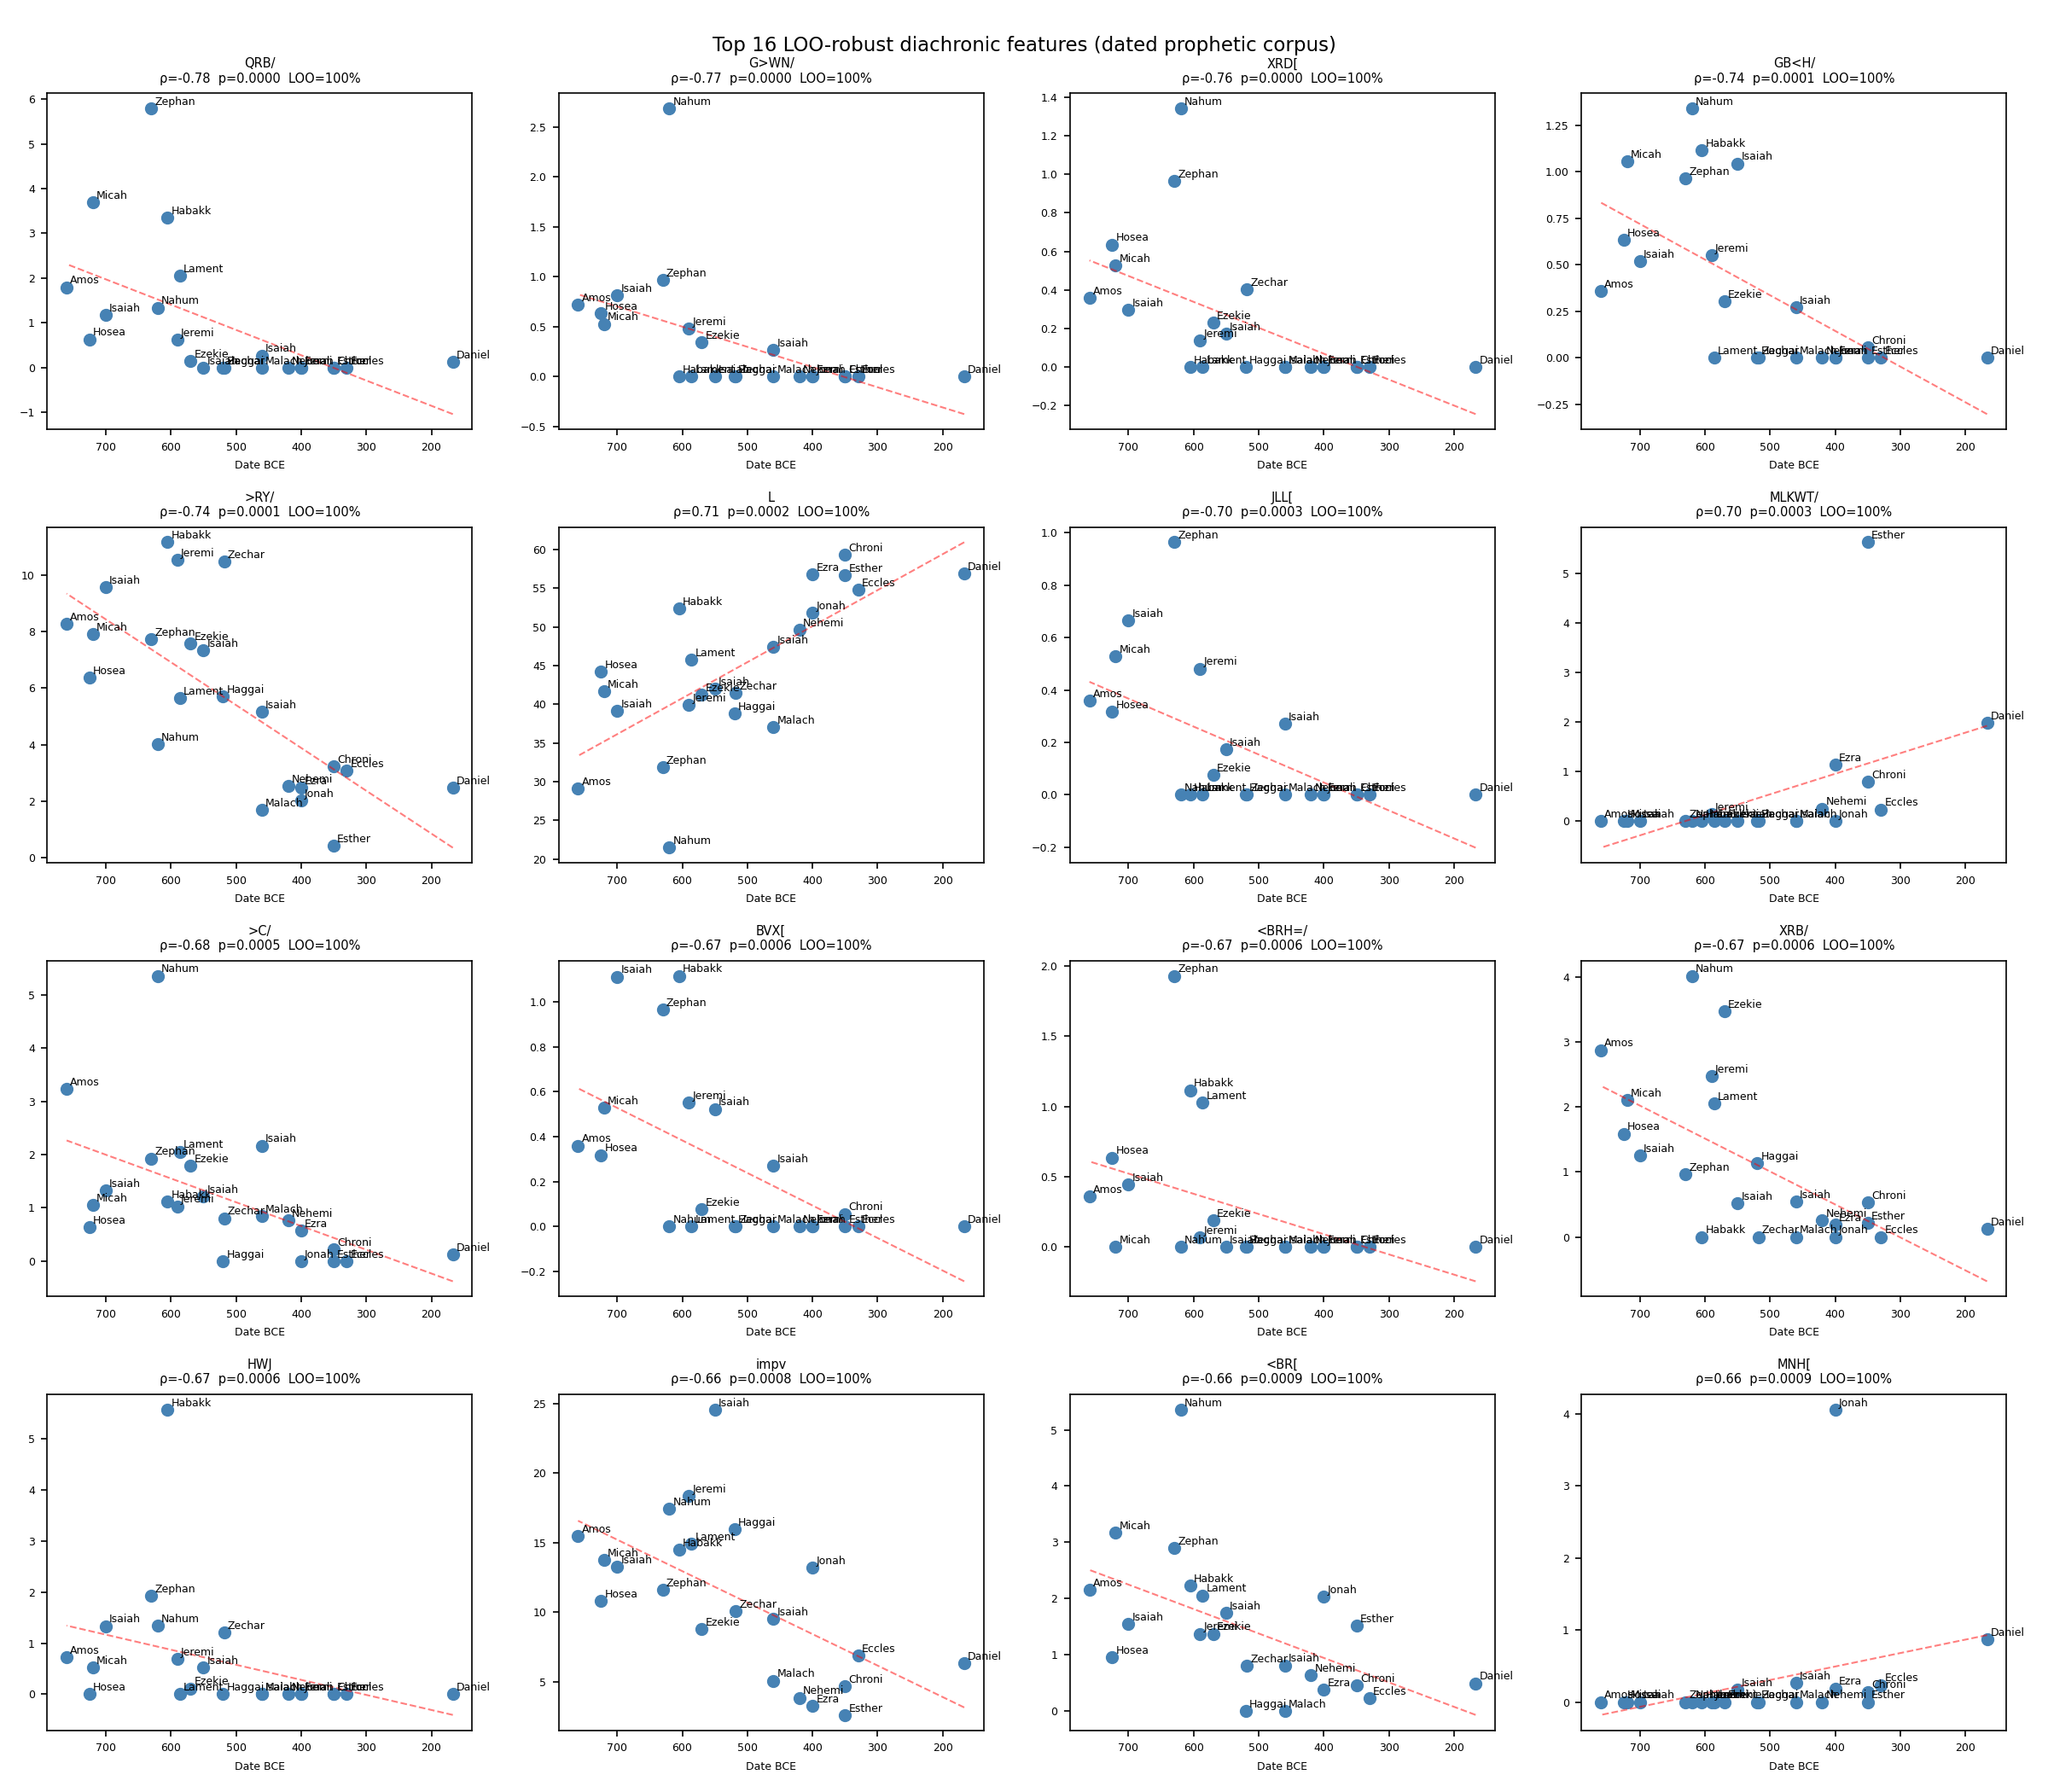
\includegraphics[width=\linewidth]{figures/fig2_feature_correlations.png}
\caption{\textbf{Top-10 morphosyntactic features by Spearman $|\rho|$
with date.}
Each panel shows the rate of one feature (y-axis) versus date BCE (x-axis)
across the 22 training units, with OLS regression line and 95\% confidence
band.  Features are color-coded by tier (Tier~1~=~lexical,
Tier~2~=~morphological, Tier~3~=~clause/phrase resistant).  The
\textit{ank\={\i}/an\={\i}} ratio and wayyiqtol fraction show the steepest
monotonic declines; infinitive-construct fraction (Tier~3) shows the most
scatter but is retained as a resistant-model feature.}
\label{fig:feature_correlations}
\end{figure}

\begin{figure}[!h]

\includegraphics[width=\linewidth]{figures/fig3_oracle_jeremiah.png}
\caption{\textbf{Oracle Jeremiah validation: full and resistant model
posteriors.}
Both the full model (35 features) and the resistant model (4 Tier-3
features) are applied to the oracle Jeremiah chapters, which were excluded
from training.  Shaded bands indicate 68\% and 95\% HDCIs.  The full-model
MAP (562~BCE) and the resistant-model MAP (538~BCE) agree within 24~yr,
confirming the oracle chapters carry no archaizing signal.
The Deuteronomistic prose stratum (Jer\_DTR, also held out) is shown for
comparison.}
\label{fig:oracle_jeremiah}
\end{figure}

\begin{figure}[!h]
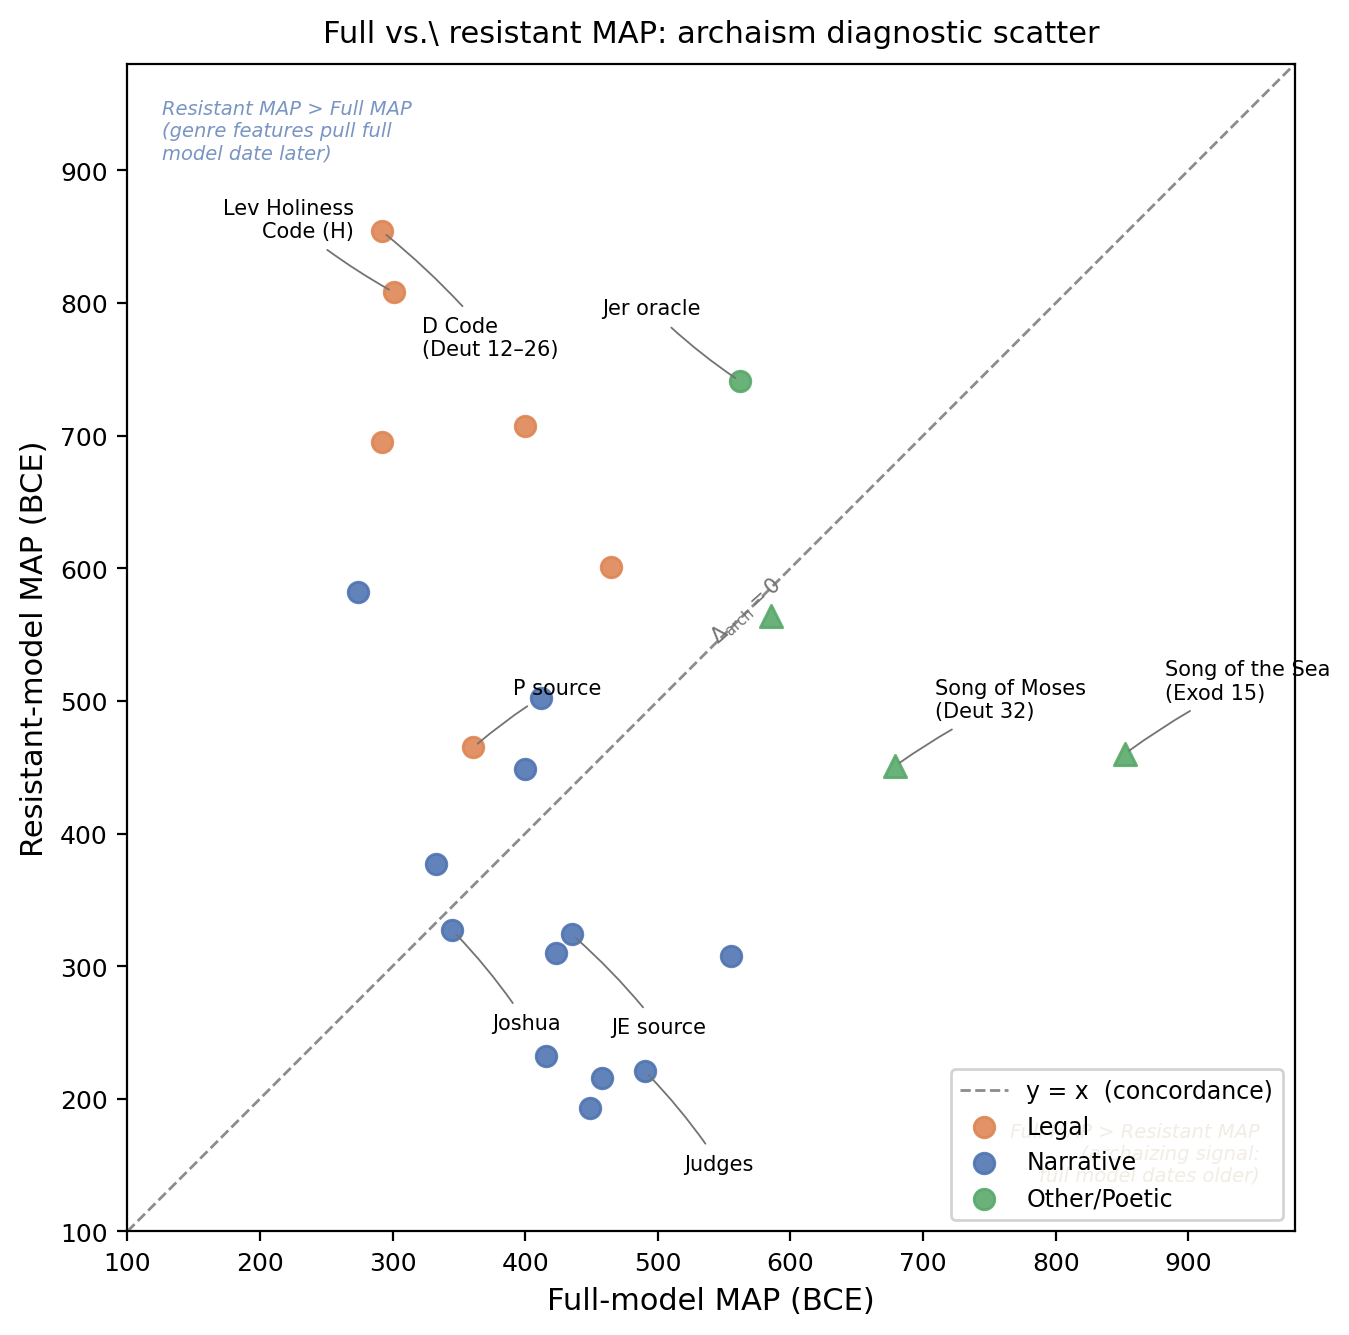
\includegraphics[width=\linewidth]{figures/fig4_full_vs_resistant.png}
\caption{\textbf{Full versus resistant MAP dates: archaism diagnostic
scatter plot.}
Each of 23 analyzed textual units is plotted with full-model MAP (x-axis)
versus resistant-model MAP (y-axis).  The diagonal reference line
indicates concordance (full~=~resistant).  Points above the diagonal
(full older than resistant) indicate archaizing composition; points below
indicate transmission-with-updating.  Song of the Sea (Exod~15) and
D\_Code (Deut~12--26) are labeled as the most extreme positive and
negative outliers, respectively.}
\label{fig:archaism_scatter}
\end{figure}

\begin{figure}[!h]

\includegraphics[width=\linewidth]{figures/fig5_genre_ratio.png}
\caption{\textbf{Genre sensitivity of the 35 morphosyntactic features.}
Features are ranked by genre ratio $\gamma_j$ (between-genre variance as
a fraction of temporal variance).  Features to the right of the dashed
threshold ($\gamma_j > 0.20$) are down-weighted in Strategy~B genre
correction.  The 12 features selected for the genre-neutral sub-model
are highlighted; these carry primarily temporal signal.}
\label{fig:genre_ratio}
\end{figure}

\begin{figure}[!h]

\includegraphics[width=\linewidth]{figures/fig6_genre_correction.png}
\caption{\textbf{Genre correction (Strategy B+D): full model versus
corrected MAP dates.}
Each bar shows the full-model MAP (gray) and B+D-corrected MAP (color) for
Torah books and selected non-prophetic texts.  Legal texts (Deuteronomy,
Leviticus) shift older under correction; narrative texts (Genesis, Numbers)
shift modestly; prophetic texts are near-zero.  The rightmost panel
compares genre-neutral MAP (open circles) to B+D MAP for legal texts,
showing the large genre contamination for D and the convergence for P.}
\label{fig:genre_correction}
\end{figure}

\begin{figure}[!h]
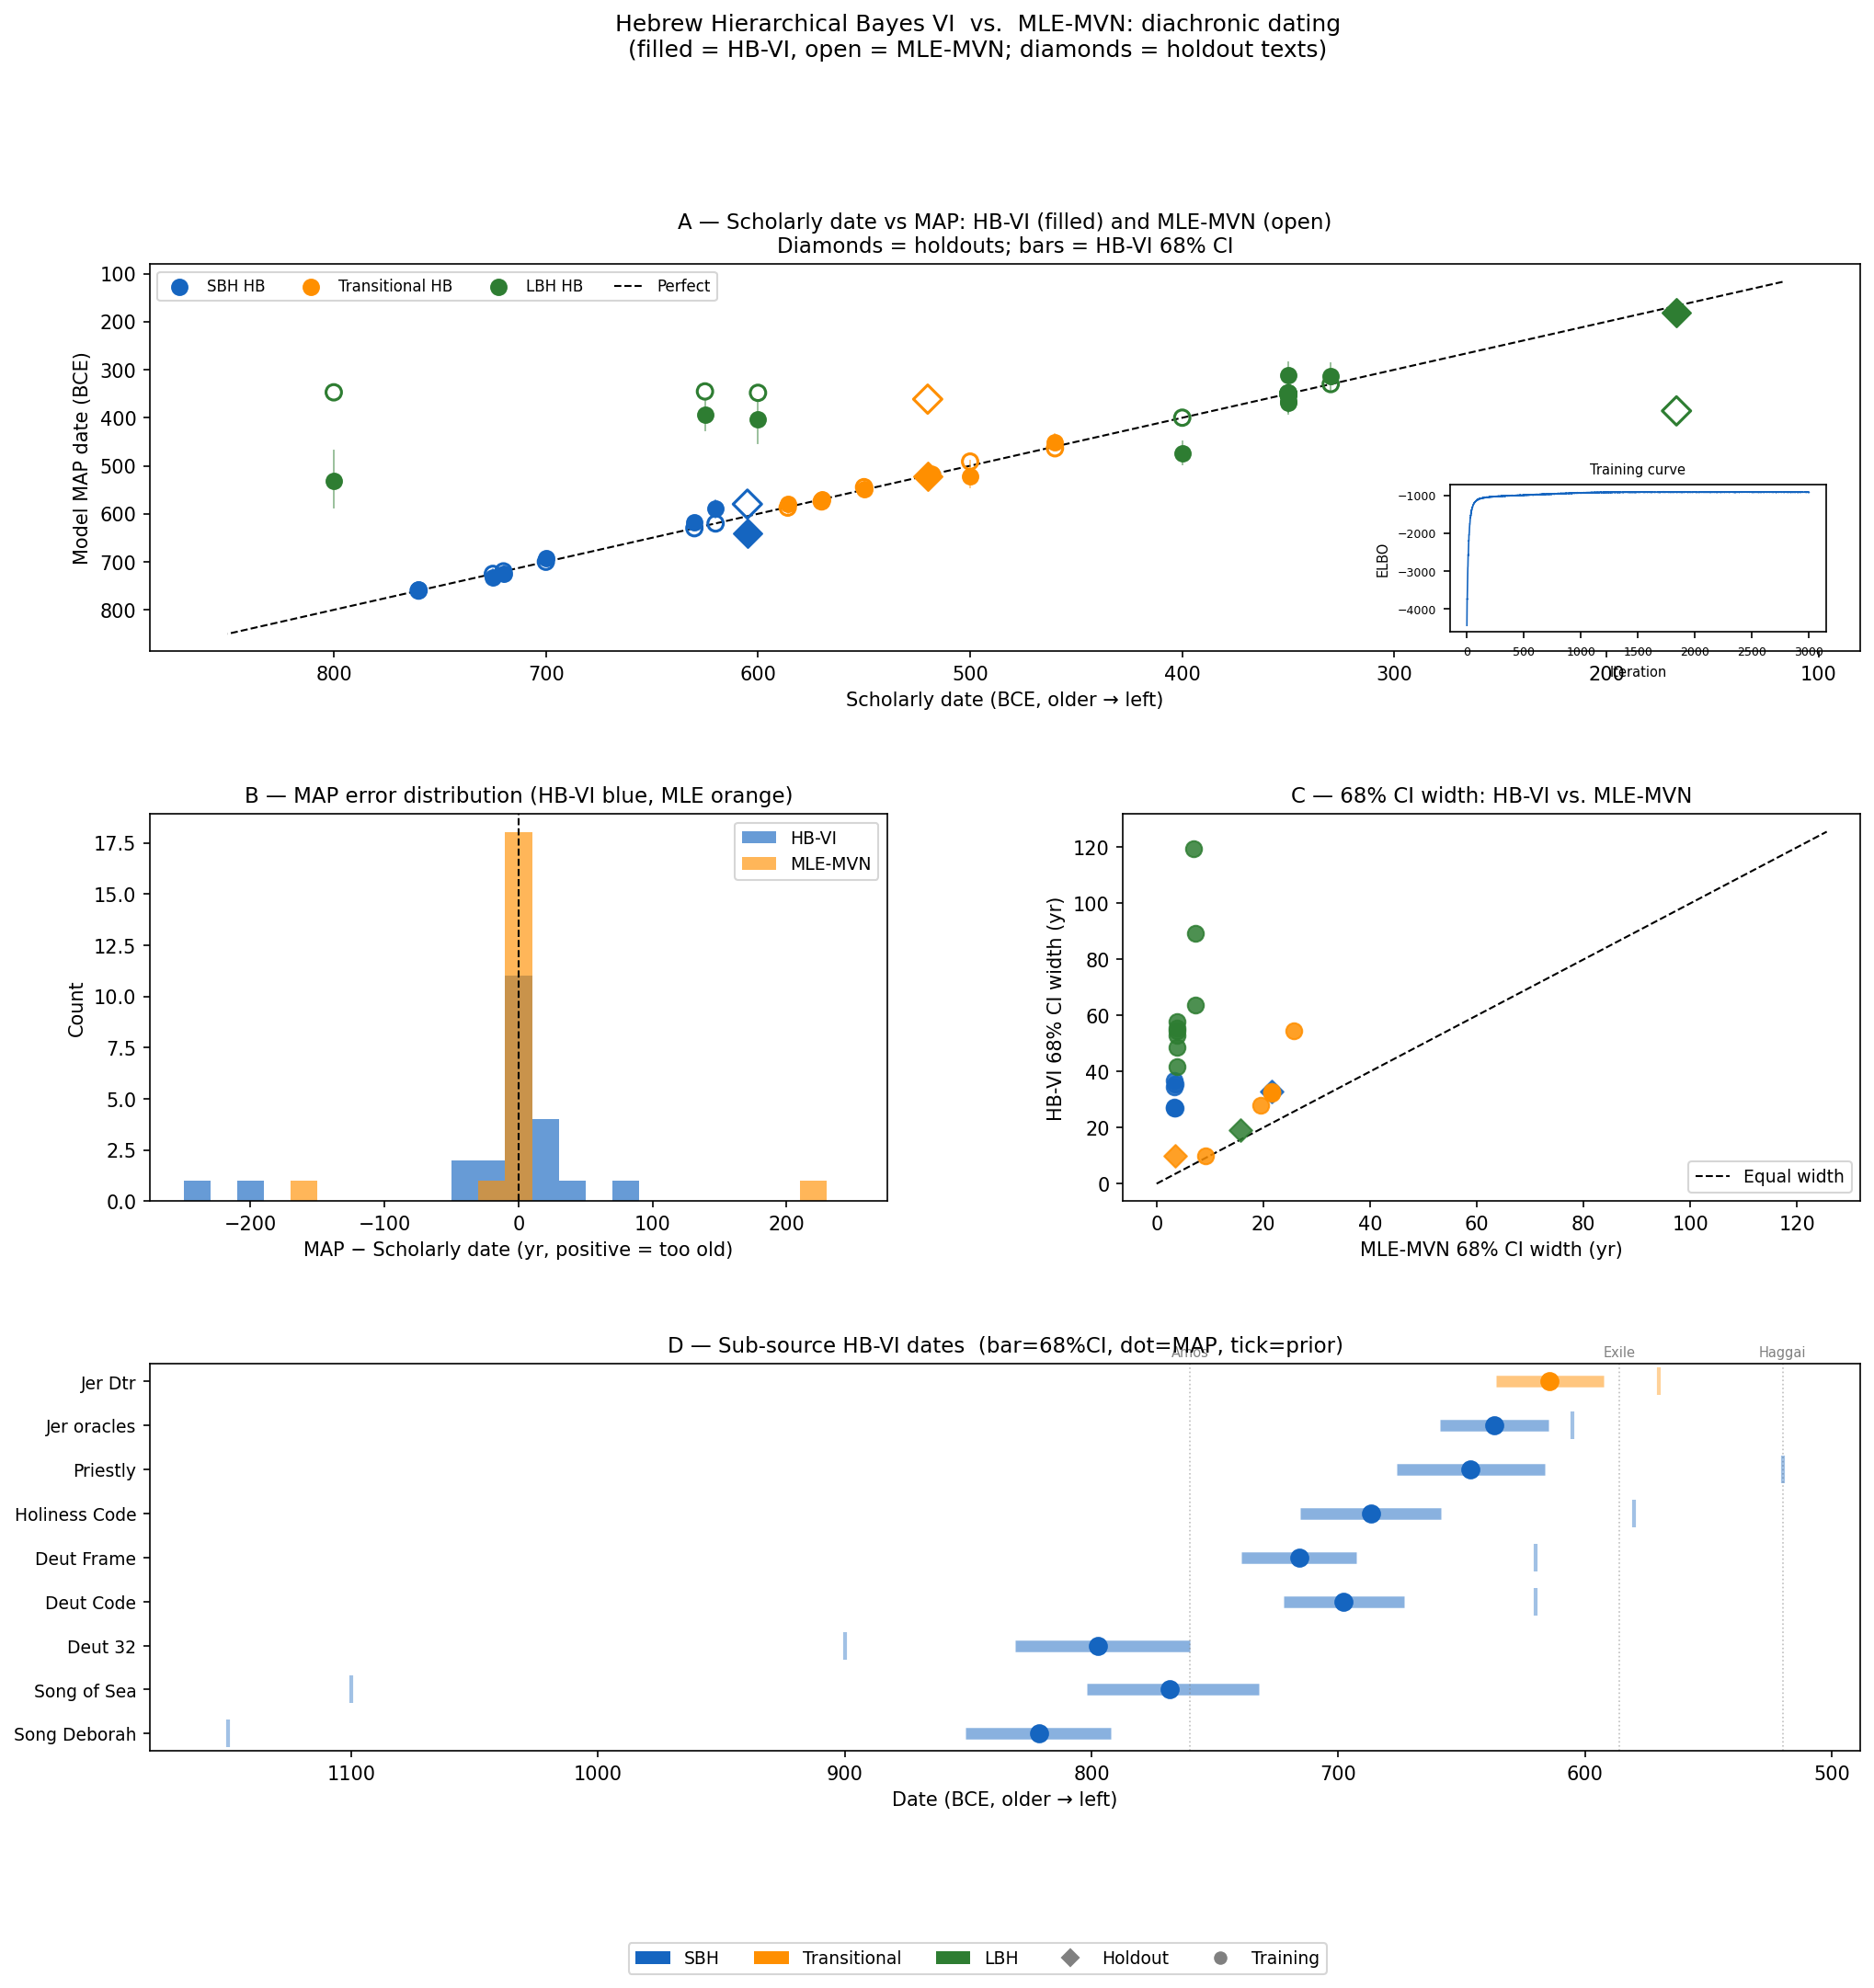
\includegraphics[width=\linewidth]{figures/fig7_hbvi_comparison.png}
\caption{\textbf{HB-VI versus MLE-MVN: MAP dates and 68\% credible
intervals for all training and comparison texts.}
Connected pairs of dots show \mvn{} (triangles) and \hbvi{} (circles) MAP
dates for each text; vertical bars indicate 68\% HDCIs.  The comparison
texts (Habakkuk, Haggai, Daniel; shaded region) illustrate the key
improvement: \hbvi{} correctly assigns Haggai to the Transitional group
(MAP~=~522~BCE) while \mvn{} miscategorizes it as LBH (MAP~=~361~BCE).
\hbvi{} CIs are systematically wider and better-calibrated than \mvn{}
CIs.}
\label{fig:hbvi_comparison}
\end{figure}

\begin{figure}[!h]
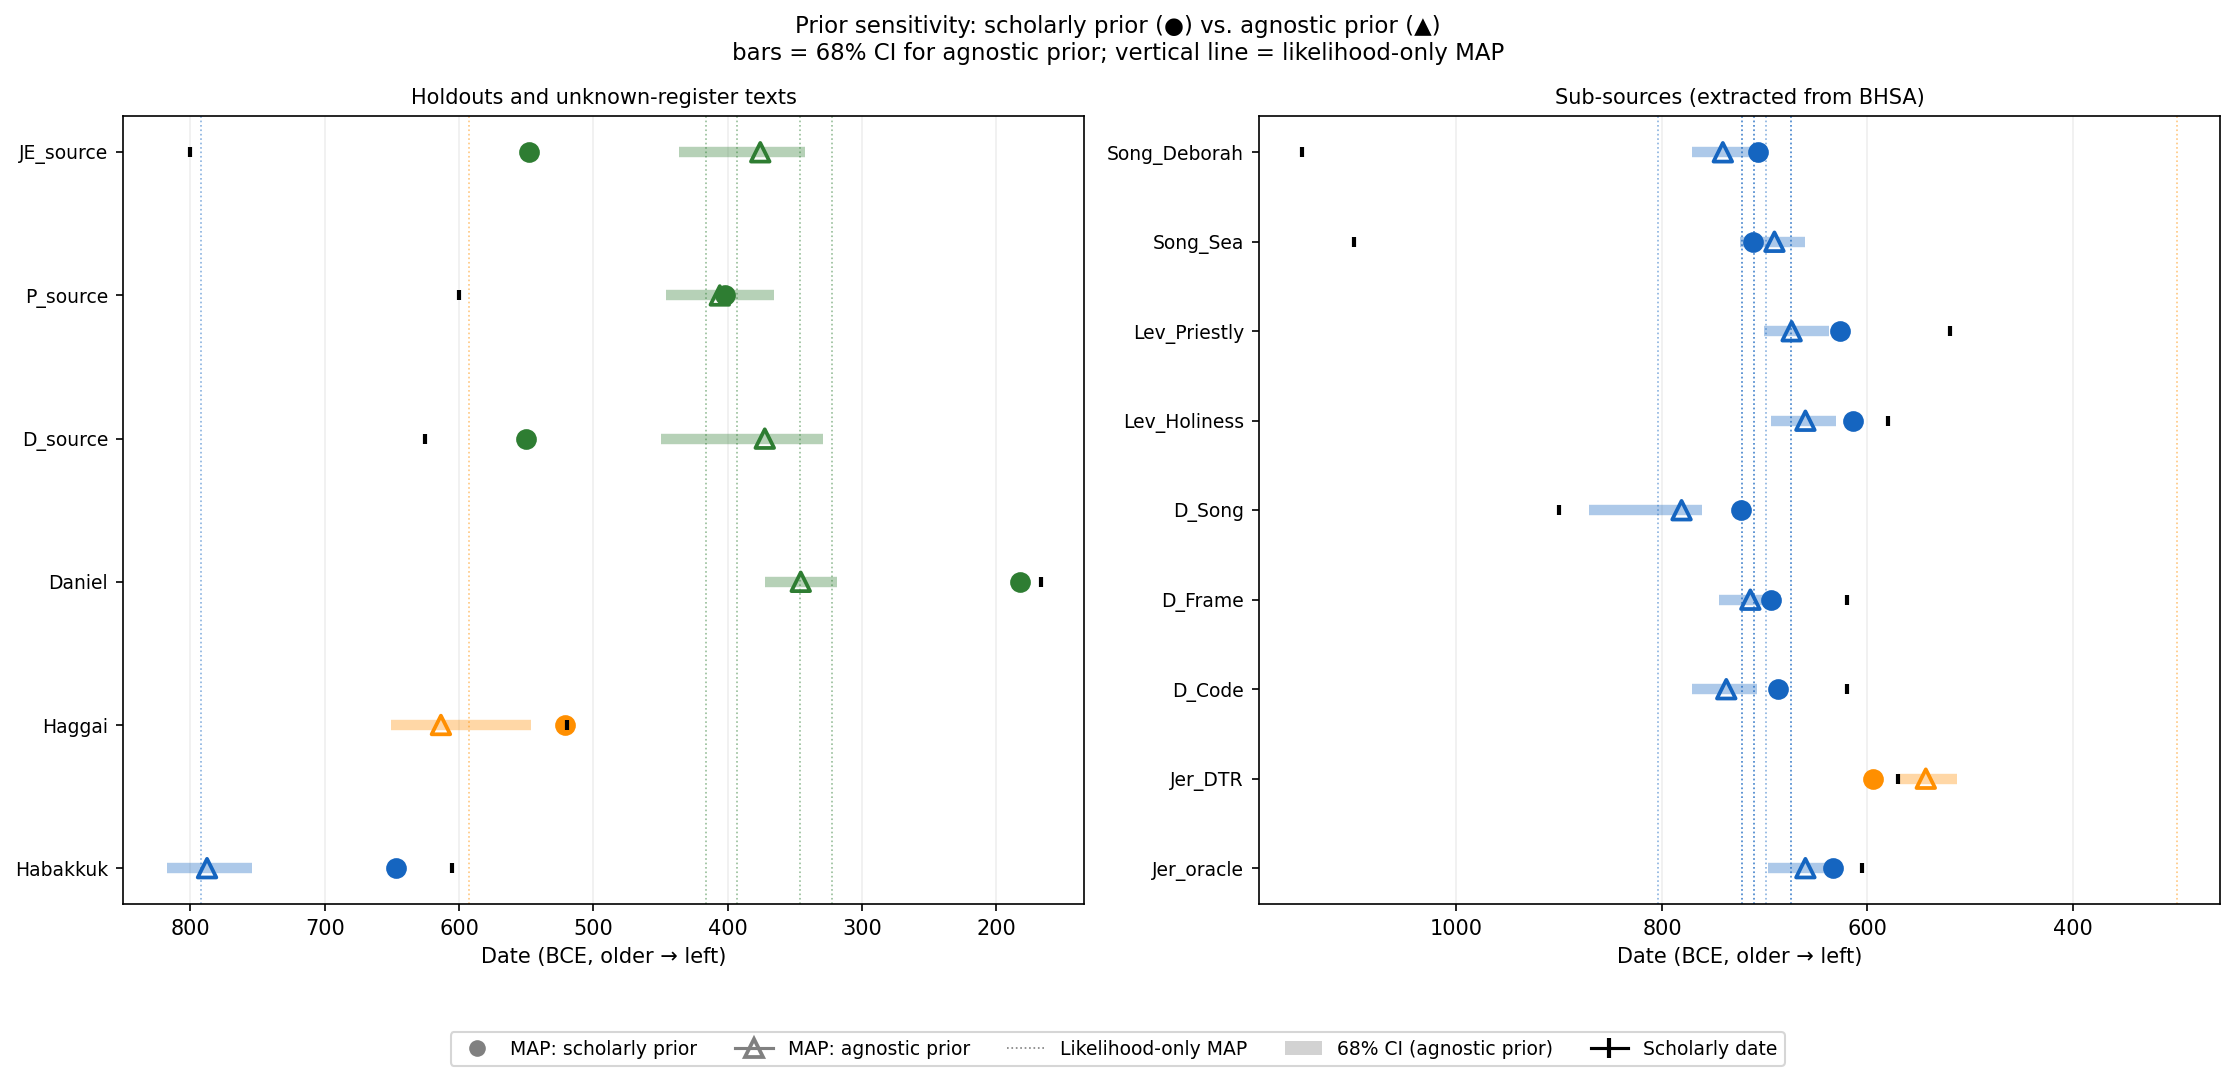
\includegraphics[width=\linewidth]{figures/fig8_prior_sensitivity.png}
\caption{\textbf{Prior sensitivity analysis: Mode~A versus Mode~B MAP
dates for all sub-sources.}
Mode~A (scholarly prior, circles) and Mode~B (agnostic prior, triangles)
MAP dates are connected for each text.  Line length represents the
$\Delta_{AB}$ shift; texts are colored by classification:
green~=~data-driven ($|\Delta_{AB}|{<}30$~yr),
orange~=~mildly prior-influenced (30--80~yr),
red~=~prior-dominated ($>80$~yr).
The four data-driven texts (Song\_Sea, P\_source, D\_Frame, Jer\_oracle)
are annotated.}
\label{fig:prior_sensitivity}
\end{figure}

\begin{figure}[!h]

\includegraphics[width=\linewidth]{figures/fig9_greek_validation.png}
\caption{\textbf{Cross-language validation on Ancient Greek (five
holdouts).}
Each holdout is plotted at its independently established date (x-axis)
versus the \mvn{} MAP date (y-axis) with 68\% CI whiskers.  All five
holdouts fall within $\sim$30~yr of the diagonal.  Register class
(ancient Attic, Koine, LXX, Atticizing) is indicated by symbol shape.
The inset shows the LXX register diagnostic features for Mark and Luke,
confirming the Semitic-substrate signal is correctly isolated from the
temporal signal.}
\label{fig:greek_validation}
\end{figure}

% -------------------------------------------------------
\bibliography{references}
% -------------------------------------------------------

\end{document}
